\chapter[Reconstruction of clonal evolution of microsatellite instability]{Reconstruction of clonal evolution of microsatellite instability\footnote{This chapter previously published as: Bonneville R, \textit{et al}. Characterization of clonal evolution in microsatellite unstable metastatic cancers through multiregional tumor sequencing. \textit{Molecular Cancer Research} 2021, 19(3):465--74.}}
\label{ch:msiclones}

%will need to cross-ref intro (maybe msi slippage figure specifically), mantis, 303 chapters
\section{Introduction}
Microsatellite instability (MSI) arises from defects in the mismatch repair (MMR) system, which includes MSH2, MSH6, MLH1 and PMS2 \cite{strand1993}. Defects in MMR may occur sporadically, for instance via \textit{MLH1} promoter hypermethylation \cite{kane1997}, or be inherited, such as in Lynch syndrome \cite{lynch1966}. MSI-H (microsatellite instability-high) is known to occur frequently in colorectal and endometrial cancer \cite{watson1994}, and has been described in multiple other cancer types \cite{bonneville2017} (Section~\ref{ssec:msilandscape:landscape_results}). During DNA replication, DNA polymerases are prone to slippage in microsatellite regions, which are short (10--60 bp), repetitive segments of DNA found throughout the human genome. This slippage erroneously adds or removes repeat units, which if uncorrected by MMR leads to MSI, or variable microsatellite lengths among affected cells.

Cancers have been increasingly recognized to comprise collections of heterogeneous malignant cells of divergent clonal ancestries, which ultimately arose from a single neoplastic ancestor \cite{gerlinger2012}. Thus, genetically distinct tumor cell populations, or subclones, may develop at different times in different regions of the body. Understanding tumor heterogeneity is important for modeling the evolution and diversification of tumor cells over time while under the influences of carcinogenesis and selective pressures. For instance, heterogeneity may result in tumor subclones with variable metastatic potential \cite{hong2015} or treatment resistance \cite{mcgranahan2017}. The presence of tumor heterogeneity also complicates diagnostic testing, as prognostic and predictive biomarkers may be found in some tumor cells but not others \cite{gerashchenko2013}, and tumor biopsies represent only a small portion of a single tumor region \cite{stanta2016}. Since tumor mutations serve as potential neoantigen targets for the immune system, subclonal mutations may contribute to differential sensitivity to immunotherapies \cite{lu2016}.

Multiple computational methods have been developed to detect MSI-H utilizing next-generation sequencing (NGS) data, such as mSINGS \cite{salipante2014} and MANTIS \cite{kautto17} (Chapter~\ref{ch:msilandscape}). Many of these sequencing-based methods have demonstrated superiority over the traditional methods of MSI-PCR \cite{boland1998}, which assays the lengths of 5--7 microsatellite loci, and MMR immunohistochemistry (IHC), which measures the expression of the MSH2, MSH6, MLH1, and PMS2 proteins. In addition, modern NGS permits detailed analysis of tumor heterogeneity. Whole exome sequencing (WES) of multiple tumors from the same patient enables characterization of subclonal tumor populations and inference of tumor evolution \cite{savas2016,chen2019,krook2019_mcs} through utilization of software tools such as PyClone \cite{roth2014}, THetA \cite{oesper2013}, SuperFreq \cite{flensburg2020} and Canopy \cite{canopy}.

However, despite these recent NGS-powered breakthroughs in both MSI-H testing of individual tumor biopsies and in analysis of tumor heterogeneity using WES of multiple tumor samples, the subclonal genomic heterogeneity in MSI-H tumors remains uncharacterized. Furthermore, the success of immunotherapy in MMR deficient cancers has attracted particular interest in the biology of MSI-H tumors, as recent studies have demonstrated that MSI-H tumors exhibit increased sensitivity and durable response rates to immune checkpoint inhibitors \cite{le2015}. A better understanding of clonality in MSI-H tumors is important for improved diagnostic testing, tumor sampling, identification and selection of tumor antigen targets for therapy, and prediction of which patients are likely to respond to immunotherapy. In this study, we examine subclonal tumor evolution with respect to mutations and microsatellites in six patients with MSI-H malignancies. We show that MMRd generates a substantial degree of tumor heterogeneity, which is reflected both in subclonal microsatellites and single nucleotide variants, and that microsatellite instability follows subclonal evolution.

\section{Materials and Methods}

\subsection{Sample acquisition and sequencing}
\label{ssec:msiclones:sampleseq}
Written informed consent was obtained from all six patients for participation in an IRB-approved study for high-throughput sequencing of tumor and normal specimens (OSU-13053, NCT02090530) at the James Cancer Hospital and The Ohio State University. This study was conducted in accordance with the Declaration of Helsinki. Frozen tumor specimens were obtained from tumor biopsies performed at The Ohio State University, formalin-fixed paraffin-embedded (FFPE) biopsy and surgical specimens were obtained from pathology archives at The Ohio State University and the Mayo Clinic, and matched normal blood samples were collected from each patient. Tumor samples were reviewed for tumor content by a board-certified pathologist.

%much of this to be replaced with cross-ref to previous chapters, moved there if necessary
Genomic DNA was extracted as previously described \cite{chen2019}, from frozen tumor biopsy samples using the \mbox{QIAamp} DNA Mini Kit (Qiagen), from FFPE specimens using the \mbox{QIAamp} DNA FFPE Tissue Kit (Qiagen), and from matched normal blood samples using the \mbox{QIAamp} DNA Blood Mini Kit (Qiagen). Libraries were prepared using the KAPA HyperPrep Kit (Roche), and were then enriched using the xGen Exome Research Panel v1.0 from IDT, supplemented with the xGen CNV Backbone Panel and a 198-probe in-house MSI panel. Paired-end whole exome sequencing (2\texttimes{}150 bp) was performed on an Illumina HiSeq 4000 at the Genomics Services Laboratory at Nationwide Children's Hospital (Columbus, Ohio).

Raw FASTQ files were aligned to the hg19 human genome \cite{lander2001} using BWA version 0.7.14 \cite{bwa} with the ``mem'' algorithm, run on the Owens supercomputer at the Ohio Supercomputer Center \cite{Owens2016}. Duplicate reads were removed with Picard \cite{Picard2019toolkit} version 2.3.0. Realignment around known insertions\slash{}deletions (indels) and base quality score recalibration were performed using Genome Analysis Toolkit (GATK) \cite{mckenna10} version 3.5.

\subsection{Variant and copy number calling}
Single nucleotide variants (SNVs) and indels were called using SAMtools \cite{samtools} version 1.3.1, VarScan2 \cite{varscan2} version 2.3.9, and bam-readcount \cite{bamreadcount}, and variants were then annotated with ANNOVAR \cite{annovar} (revision \#11f4bb, 2016-02-01) as previously described \cite{chen2019} (Section~\ref{ssec:240:alignment_variant_calling}). DANN scores \cite{quang2015} were used to predict functional impact of nonsynonymous SNVs, with a threshold of 0.96 to consider a SNV deleterious. Mutational signatures were called using deconstructSigs \cite{rosenthal16} version 1.8.0 with default settings and ``exome2genome'' trinucleotide frequency correction, using the COSMIC version 2 set of 30 mutational signatures \cite{cosmic_ms}. Allele-specific copy number variations (CNVs) were called using FALCON \cite{falcon} version 0.2, followed by manual curation as previously described \cite{chen2019} (Section~\ref{ssec:240:cnv_methods}). Neighbor-joining trees based on somatic variants were generated using RapidNJ \cite{simonsen08} (Section~\ref{ssec:240:nj_methods}), and visualized with Interactive Tree of Life \cite{letunic16} (iTOL) version 4.2.3.

\subsection{Per-sample microsatellite instability analysis}
Per-sample microsatellite length distributions and microsatellite instability were called using MANTIS \cite{kautto17} version 1.0.4 run with recommended whole exome settings (Section~\ref{ssec:msilandscape:tool_params}). 2,551 microsatellite loci (Supplemental File~S\thechapter{}.1) were assessed in each sample; the union of 2,539 loci originally used by Salipante \textit{et al} \cite{salipante2014} and in our validation of MANTIS (Section~\ref{ssec:msilandscape:loci_selection}), and 99 loci targeted by our in-house MSI probe panel.

\subsection{Subclonal inference}
\label{ssec:msiclones:inference}
\begin{figure}[ht]
    \centering
    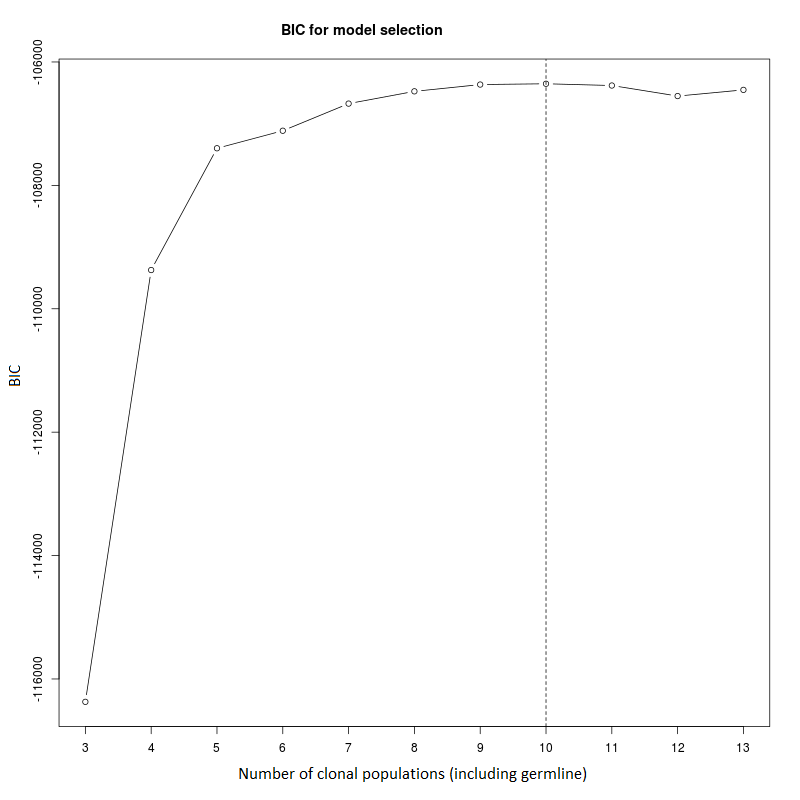
\includegraphics[width=0.6\linewidth]{images/msiclones/patient6_bic}
	\vspace{-0.3cm}
    \caption[BIC scores of subclonal models with 3--13 clonal populations in patient 6.]{BIC (Bayesian Information Criterion) scores of subclonal models with 3--13 clonal populations in patient 6. We utilized Canopy to generate phylogenetic trees of subclonal evolution with 3 to 13 clonal populations, where clonal populations include germline and tumor subclones. A nine-population (eight tumor subclones) model was manually selected (BIC = -106,366.1), as it yielded essentially equivalent BIC as the ten-population (nine tumor subclones) model favored by Canopy (BIC = -106,353.2).}
    \label{fig:msiclones:bic_5}
\end{figure}

Subclonal cancer cell populations were identified using Canopy \cite{canopy} as previously described \cite{chen2019} (Section~\ref{ssec:240:canopy_tree}). After selection of ultra-high-confidence SNVs, these sets of SNVs were downsampled to 60 SNVs utilizing a high correlation filter for patients 2, 5, and 6 (Section~\ref{ssec:303:phylo_analysis}). Canopy \cite{canopy} failed to generate a tree with 60 SNVs for patient 3, therefore 400 SNVs were used for patient 3. As only 195 SNVs passed the ultra-high-confidence filters in patient 1 and 137 SNVs in patient 4, these SNVs were not downsampled. Ultra-high-confidence SNVs, and the CNVs called by FALCON \cite{falcon} and manually curated, were used as input for Canopy for patient 6. Canopy was run with SNVs only for patients 1--5, as no CNVs in those patients passed curation. In addition, rather than utilizing the Frobenius norm of the $\varepsilon_M$ and $\varepsilon_m$ matrices from FALCON \cite{falcon}, missing values in these matrices were imputed using the R package \texttt{missForest} with default settings \cite{missForest}. For all six patients, the maximum permitted simulation runs was increased to at least 100,000, and the maximum permitted subclones increased to 12. This procedure resulted in phylogenetic trees of tumor subclones, along with the estimated prevalence of each subclone in each tumor sample. We attempted to remove the hysterectomy sample from patient 5 due to its poor tumor purity (10--20\%), however Canopy failed to find a tree without it, likely due to lack of clonal diversity among the other patient 5 samples. The number of subclones yielding the lowest BIC (Bayesian Information Criterion) score was selected for patients 1--5, however for patient 6 an eight-subclone model was manually chosen due to its comparable BIC with the optimal nine-subclone model (Figure~\ref{fig:msiclones:bic_5}). Note that subclones were not renumbered, therefore subclone numbers do not necessarily correspond to evolutionary relationships. After trees were generated, we performed \textit{post hoc} assignment of the remaining SNVs (not used by Canopy for tree-building) and indels (Section~\ref{ssec:240:tree_assignment}) as well as estimating temporal ordering of mutations (Section~\ref{ssec:240:mutational_ordering}) in each patient as previously described \cite{krook2019_mcs}.

\subsection{Analysis of subclonal microsatellite instability}
\label{ssec:msiclones:subclonal_msi}
Within a single patient, define $K$ as the number of \mbox{subclones + 1} (germline), with $k=1$ corresponding to germline (hereafter considered as an independent subclone). Define $N$ as the number of samples. Therefore, we have a matrix $\mathbf{P} \in \mathbb{R}^{K \times N}$, representing the fraction of normal for $k=1$ and subclone $k-1$ for $k \in 2 \twodots K$ in sample $i \in 1 \twodots N$. $\mathbf{P}$ is obtained directly from Canopy output.

Consider a single microsatellite locus $r \in R$, the set of all microsatellite loci sufficiently covered in all tumor samples from this patient for MANTIS to score. $g(l)$ represents the empirical pmf (probability mass function) of microsatellite lengths $l$ observed in the germline (from matched normal sequencing). $h_i(l)$ represents the empirical pmf of microsatellite lengths observed in sample $i$. Both $g(l)$ and all $h_i(l)$ are obtained directly from MANTIS output. To be estimated for this locus is $f_k(l)$, the pmfs of microsatellite lengths for all subclones $k \in 2 \twodots K$.

As the domain of $h_i(l)$ is a finite set (the different number of microsatellite lengths observed in at least one tumor sample at this locus), its range for each $i$ can be collected into a matrix $\mathbf{D} \in \mathbb{R}^{L \times N}$, where $L$ is the total number of observed lengths of this microsatellite, as follows:
\[
	\mathbf{D} = 
	\begin{bmatrix}
	h_1(l_1) & h_2(l_1) & \dots & h_N(l_1)\\
	h_1(l_2) & h_2(l_2) & \dots & h_N(l_2)\\
	\dots    & \dots    & \dots & \dots   \\
	h_1(l_L) & h_2(l_L) & \dots & h_N(l_L)
	\end{bmatrix}
\]

If $r$ is located within a CNV-affected region, $\mathbf{P}$ must be adjusted to account for the different relative contributions of each subclone to this region. Define $T$ as the set of CNV-affected regions. From Canopy, we have the per-subclone major copy matrix $\mathbf{\tilde{C}}^\text{M} \in \mathbb{Z}^{|T| \times K}$ and the per-subclone minor copy matrix $\mathbf{\tilde{C}}^\text{m} \in \mathbb{Z}^{|T| \times K}$. These sum to $\mathbf{\tilde{C}}^\text{M} + \mathbf{\tilde{C}}^\text{m} = \mathbf{\tilde{C}} \in \mathbb{Z}^{|T| \times K}$, the per-subclone total copy matrix. For each CNV-affected region $t \in T$, we compute a matrix of per-subclone total copy numbers in each sample $\mathbf{A}(t) \in \mathbb{R}^{K \times N}$ as follows:
\begin{equation}
	A_{ij}(t) = P_{ij} \tilde{C}_{ti} \qquad i = 1 \twodots K, j = 1 \twodots N
\end{equation}
For a microsatellite locus $r$, we compute the adjusted $\mathbf{\tilde{P}}(r) \in \mathbb{R}^{K \times N}$ as follows:
\begin{equation}
	\tilde{P}_{ij}(r) = \begin{cases}
		\frac{A_{ij}(t)}{\sum_{k=1}^{K}A_{kj}} & \text{if } \exists t \in T \text{ s.t. } r \in t \\
		P_{ij} & \text{otherwise}
	\end{cases} \qquad i = 1 \twodots K, j = 1 \twodots N
\end{equation}
If any row $\tilde{P}_{i*}$ consists entirely of zeros, which can occur with deletion of both alleles in one or more subclones, any loci in that region are excluded from further analysis as their distributions within these subclones cannot be uniquely determined.

For each locus $r$ (hereafter omitted for clarity), to be solved is a matrix $\mathbf{M} \in \mathbb{R}^{L \times K}$, with each $M_{lk}$ representing the fraction of reads supporting microsatellite length $l$ in subclone $k$. The first column of $\mathbf{M}$, corresponding to microsatellite lengths supported by the germline, is known from $g(l)$ and fixed:
\[
	\mathbf{M}_{*1} = \begin{bmatrix} g(l_1) & g(l_2) & \dots & g(l_L) \end{bmatrix}^{\mathsf{T}}
\]
All columns of $\mathbf{M}$ must be constrained to sum to 1. Each of the remaining columns of $\mathbf{M}$ correspond to $f_k(l)$. $\mathbf{M}$ is related to known $\mathbf{\tilde{P}}$ and $\mathbf{D}$ (specific to the locus $r$) as follows:
\begin{equation}
\mathbf{M} \mathbf{\tilde{P}} \approx \mathbf{D}
\end{equation}

To be optimized is $\mathbf{M}_{lk} \text{ for } l \in 1 \twodots L, k \in 2 \twodots K$, such that
\begin{equation}
\sse(\mathbf{M} | \mathbf{\tilde{P}}, \mathbf{D}) = \lVert \mathbf{M} \mathbf{\tilde{P}} - \mathbf{D} \rVert^2_F
\end{equation}
is minimized ($\sse$ indicates the sum of squared error, and $\scriptstyle{F}$ indicates the matrix Frobenius norm). We applied simulated annealing \cite{metropolis53,kirkpatrick83} (with 50 chains and 50,000 iterations) as follows to determine an approximate optimal fit for $\hat{\mathbf{M}}$. Each column after the first corresponds to the per-subclone microsatellite length distributions most consistent with per-sample microsatellite distributions and subclonal composition, and its first column is fixed to the germline microsatellite distribution.

Given hyperparameters $\eta_0 = 0.2$ (starting learning rate), $\eta_\text{max} = 0.01$ (end learning rate), $\lambda = 0.01$ (suboptimal jump probability scaling), $\rho = 4$ (suboptimal jump suppression factor), we estimate optimal $\hat{\mathbf{M}}$ as follows:
\begin{algorithm}[H]
	\caption{Initialization}
	\label{alg:msiclones:mh-init}
	\begin{algorithmic}[1]
	\For{$i \in 1 \twodots L$}
		\For{$k \in 2 \twodots K$}
			\State $M_{lk} \gets \text{Uniform}(0, 1)$
		\EndFor
	\EndFor
	\State $\hat{\mathbf{M}} \gets \mathbf{M}$
	\For{$i \in 1 \twodots L$}
		\For{$k \in 2 \twodots K$}
			\State $M_{lk} \gets M_{lk} / \lVert \hat{\mathbf{M}}_{*k} \rVert_1$
		\EndFor
	\EndFor
	\State $\hat{\mathbf{M}} \gets \mathbf{M}$
	\end{algorithmic}
\end{algorithm}

\begin{algorithm}[H]
	\caption{Training}
	\label{alg:msiclones:mh-train}
	\begin{algorithmic}[1]
		\For{$i \in 1 \twodots 50000$}
			\State $k \gets \text{Uniform}\{2, K\}$ \Comment{Random subclone}
			\State $l_1, l_2 \gets \text{two distinct random rows of } \mathbf{M}$ \Comment{Random microsatellite lengths}
			\State $\mathbf{M}' \gets \mathbf{M}$
			\State $x \gets M_{l_1 k}, y \gets M_{l_2 k}$
			\State $s \gets {x + y}$
			\State $x \gets x/s, y \gets y/s$
			\State $\eta \gets (\eta_\text{max} - \eta_0)(t-1)(t_\text{max}-1)^{-1} + \eta_0$ \Comment{Linear learning rate decay}
			\State $\delta \gets \mathcal{N}(0, \eta)$ such that $(x + \delta) \in [0, 1]$
			\State $M'_{l_1 k} \gets s(x + \delta), M'_{l_2 k} \gets s(1 - x - \delta)$ \Comment{Randomly redistribute probabilities}
			\State $z \gets \sse(\mathbf{M} | \mathbf{\tilde{P}}, \mathbf{D})$, $z' \gets \sse(\mathbf{M}' | \mathbf{\tilde{P}}, \mathbf{D})$
			\State $r \gets \lambda (\!\frac{z}{z'}\!)^\rho$
			\State $t \gets \text{Uniform}(0, 1)$
			\IfThen{$z' < z \lor t < r$}%
				{$\mathbf{M} \gets \mathbf{M}'$} \Comment{Accept move}
			\IfThen{$z' < \sse(\hat{\mathbf{M}} | \mathbf{\tilde{P}}, \mathbf{D})$}%
				{$\hat{\mathbf{M}} \gets \mathbf{M}'$} \Comment{Save best solution}
		\EndFor
	\end{algorithmic}
\end{algorithm}%
\noindent where $\mathcal{N}(\mu, \sigma)$ is a normal distribution with mean $\mu$ and standard deviation $\sigma$. We train 50 $\hat{\mathbf{M}}$ models for each microsatellite locus, and the best-fitting $\hat{\mathbf{M}}$ for each locus is selected for further analysis (Figure~\ref{fig:msiclones:mcmc_path}).

\begin{figure}[ht]
    \begin{center}
        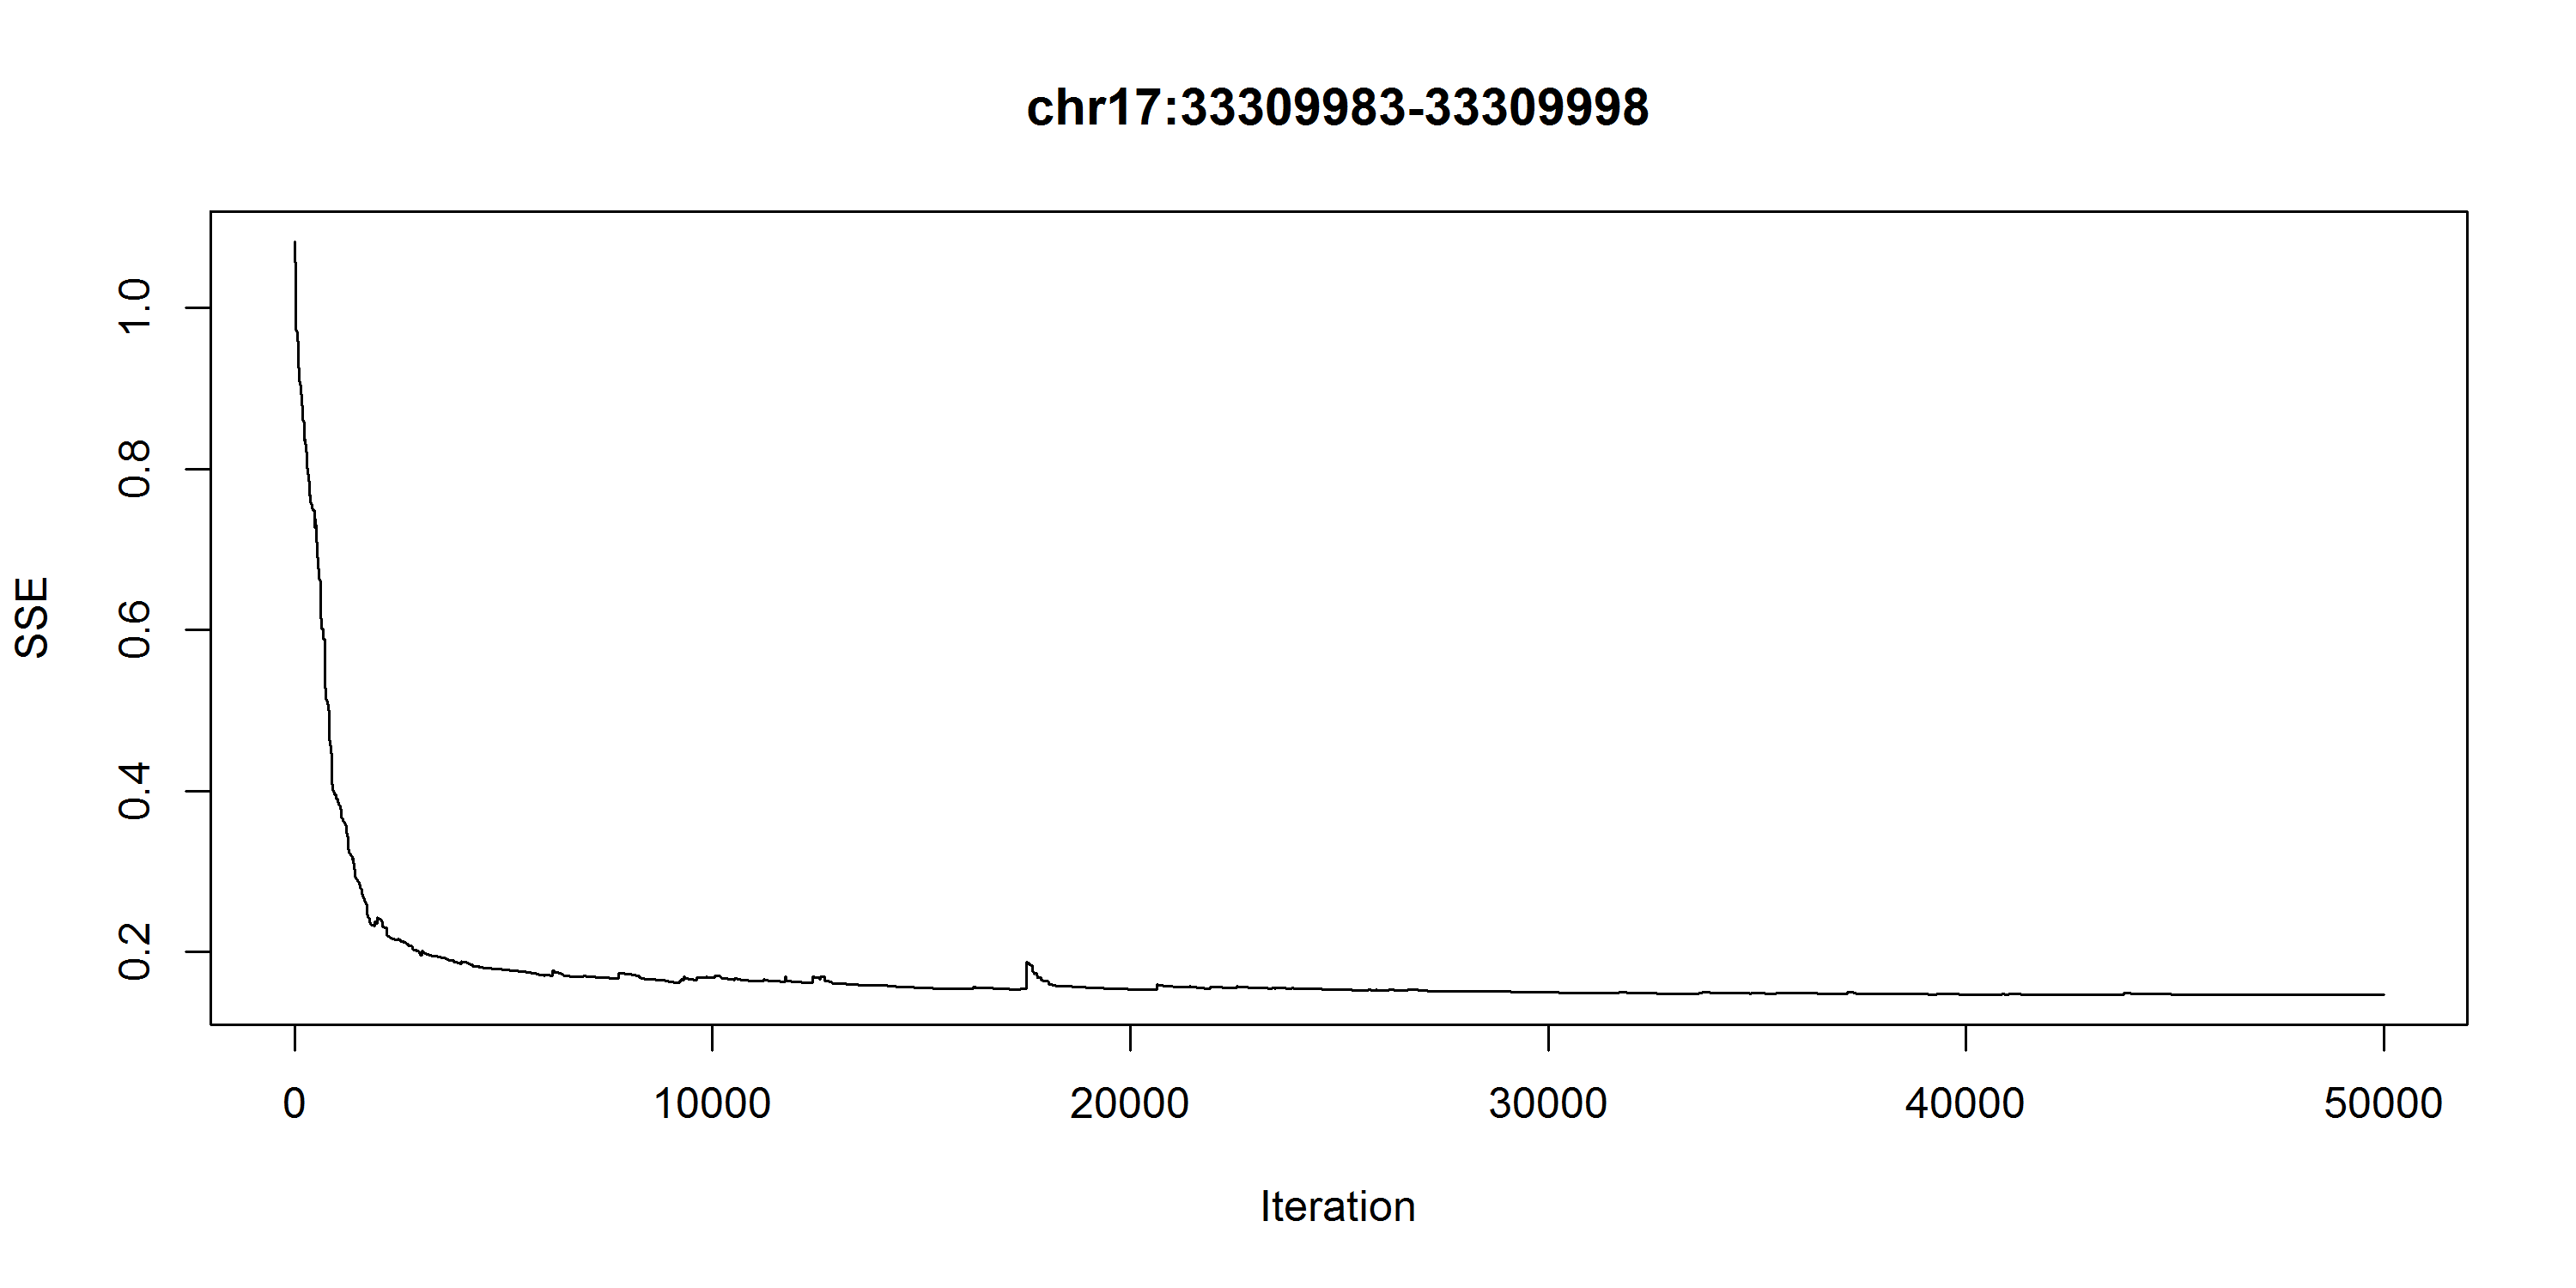
\includegraphics[width=0.95\linewidth]{images/msiclones/mcmc_path}
    \end{center}
	\vspace{-0.3cm}
    \caption[Example simulated annealing chain.]{Example simulated annealing chain from subclonal MSI inference of the microsatellite locus chr17:33309983--33309998 in patient 6 demonstrates model convergence. Y axis indicates SSE (sum of squared error), with lower SSE corresponding to better model fit at this locus.}
    \label{fig:msiclones:mcmc_path}
\end{figure}

Note that $\hat{\mathbf{M}}$ is only uniquely solvable if $K \leq N + 1$, as was true for all patients in this study. Consider for any microsatellte length $l \in L$ (for any individual locus), a reduced equation $\mathbf{M'} \mathbf{\tilde{P}'} \approx \mathbf{D'}$, in which $\mathbf{M'} \in \mathbb{R}^{1 \times K-1}$ with the first (germline) column and all but one loci rows removed from $\mathbf{M}$, $\mathbf{\tilde{P}'} \in \mathbb{R}^{K-1 \times N}$ with the first (proportion normal) row removed from $\mathbf{\tilde{P}}$, and $\mathbf{D'} \in \mathbb{R}^{1 \times N}$. This equation lacks the constraints that $\mathbf{M}_{*1}$ is fixed and that columns of $\mathbf{M}$ sum to 1. Rearranging gives $\mathbf{\tilde{P}}^{\prime \mathsf{T}} \mathbf{M}^{\prime \mathsf{T}} \approx \mathbf{D}^{\prime \mathsf{T}}$, with best $\hat{\mathbf{M}}^{\prime \mathsf{T}}$ by least-squares given by $\hat{\mathbf{M}}^{\prime \mathsf{T}} = (\mathbf{\tilde{P}'}\mathbf{\tilde{P}}^{\prime \mathsf{T}})^{-1}\mathbf{\tilde{P}'}\mathbf{D}^{\prime \mathsf{T}}$. $\mathbf{\tilde{P}'}\mathbf{\tilde{P}}^{\prime \mathsf{T}} \in \mathbb{R}^{K-1 \times K-1}$, and $\text{rank}(\mathbf{\tilde{P}'}) = \text{rank}(\mathbf{\tilde{P}'}\mathbf{\tilde{P}}^{\prime \mathsf{T}})$. If $K - 1 > N$, then $\text{rank}(\mathbf{\tilde{P}'}) \leq N$ and $\mathbf{\tilde{P}'}\mathbf{\tilde{P}}^{\prime \mathsf{T}}$ is singular, indicating an underdetermined system of equations.

\subsection{Benchmarking}
\label{ssec:msiclones:benchmarking}
\begin{figure}[htp]
	\centering
	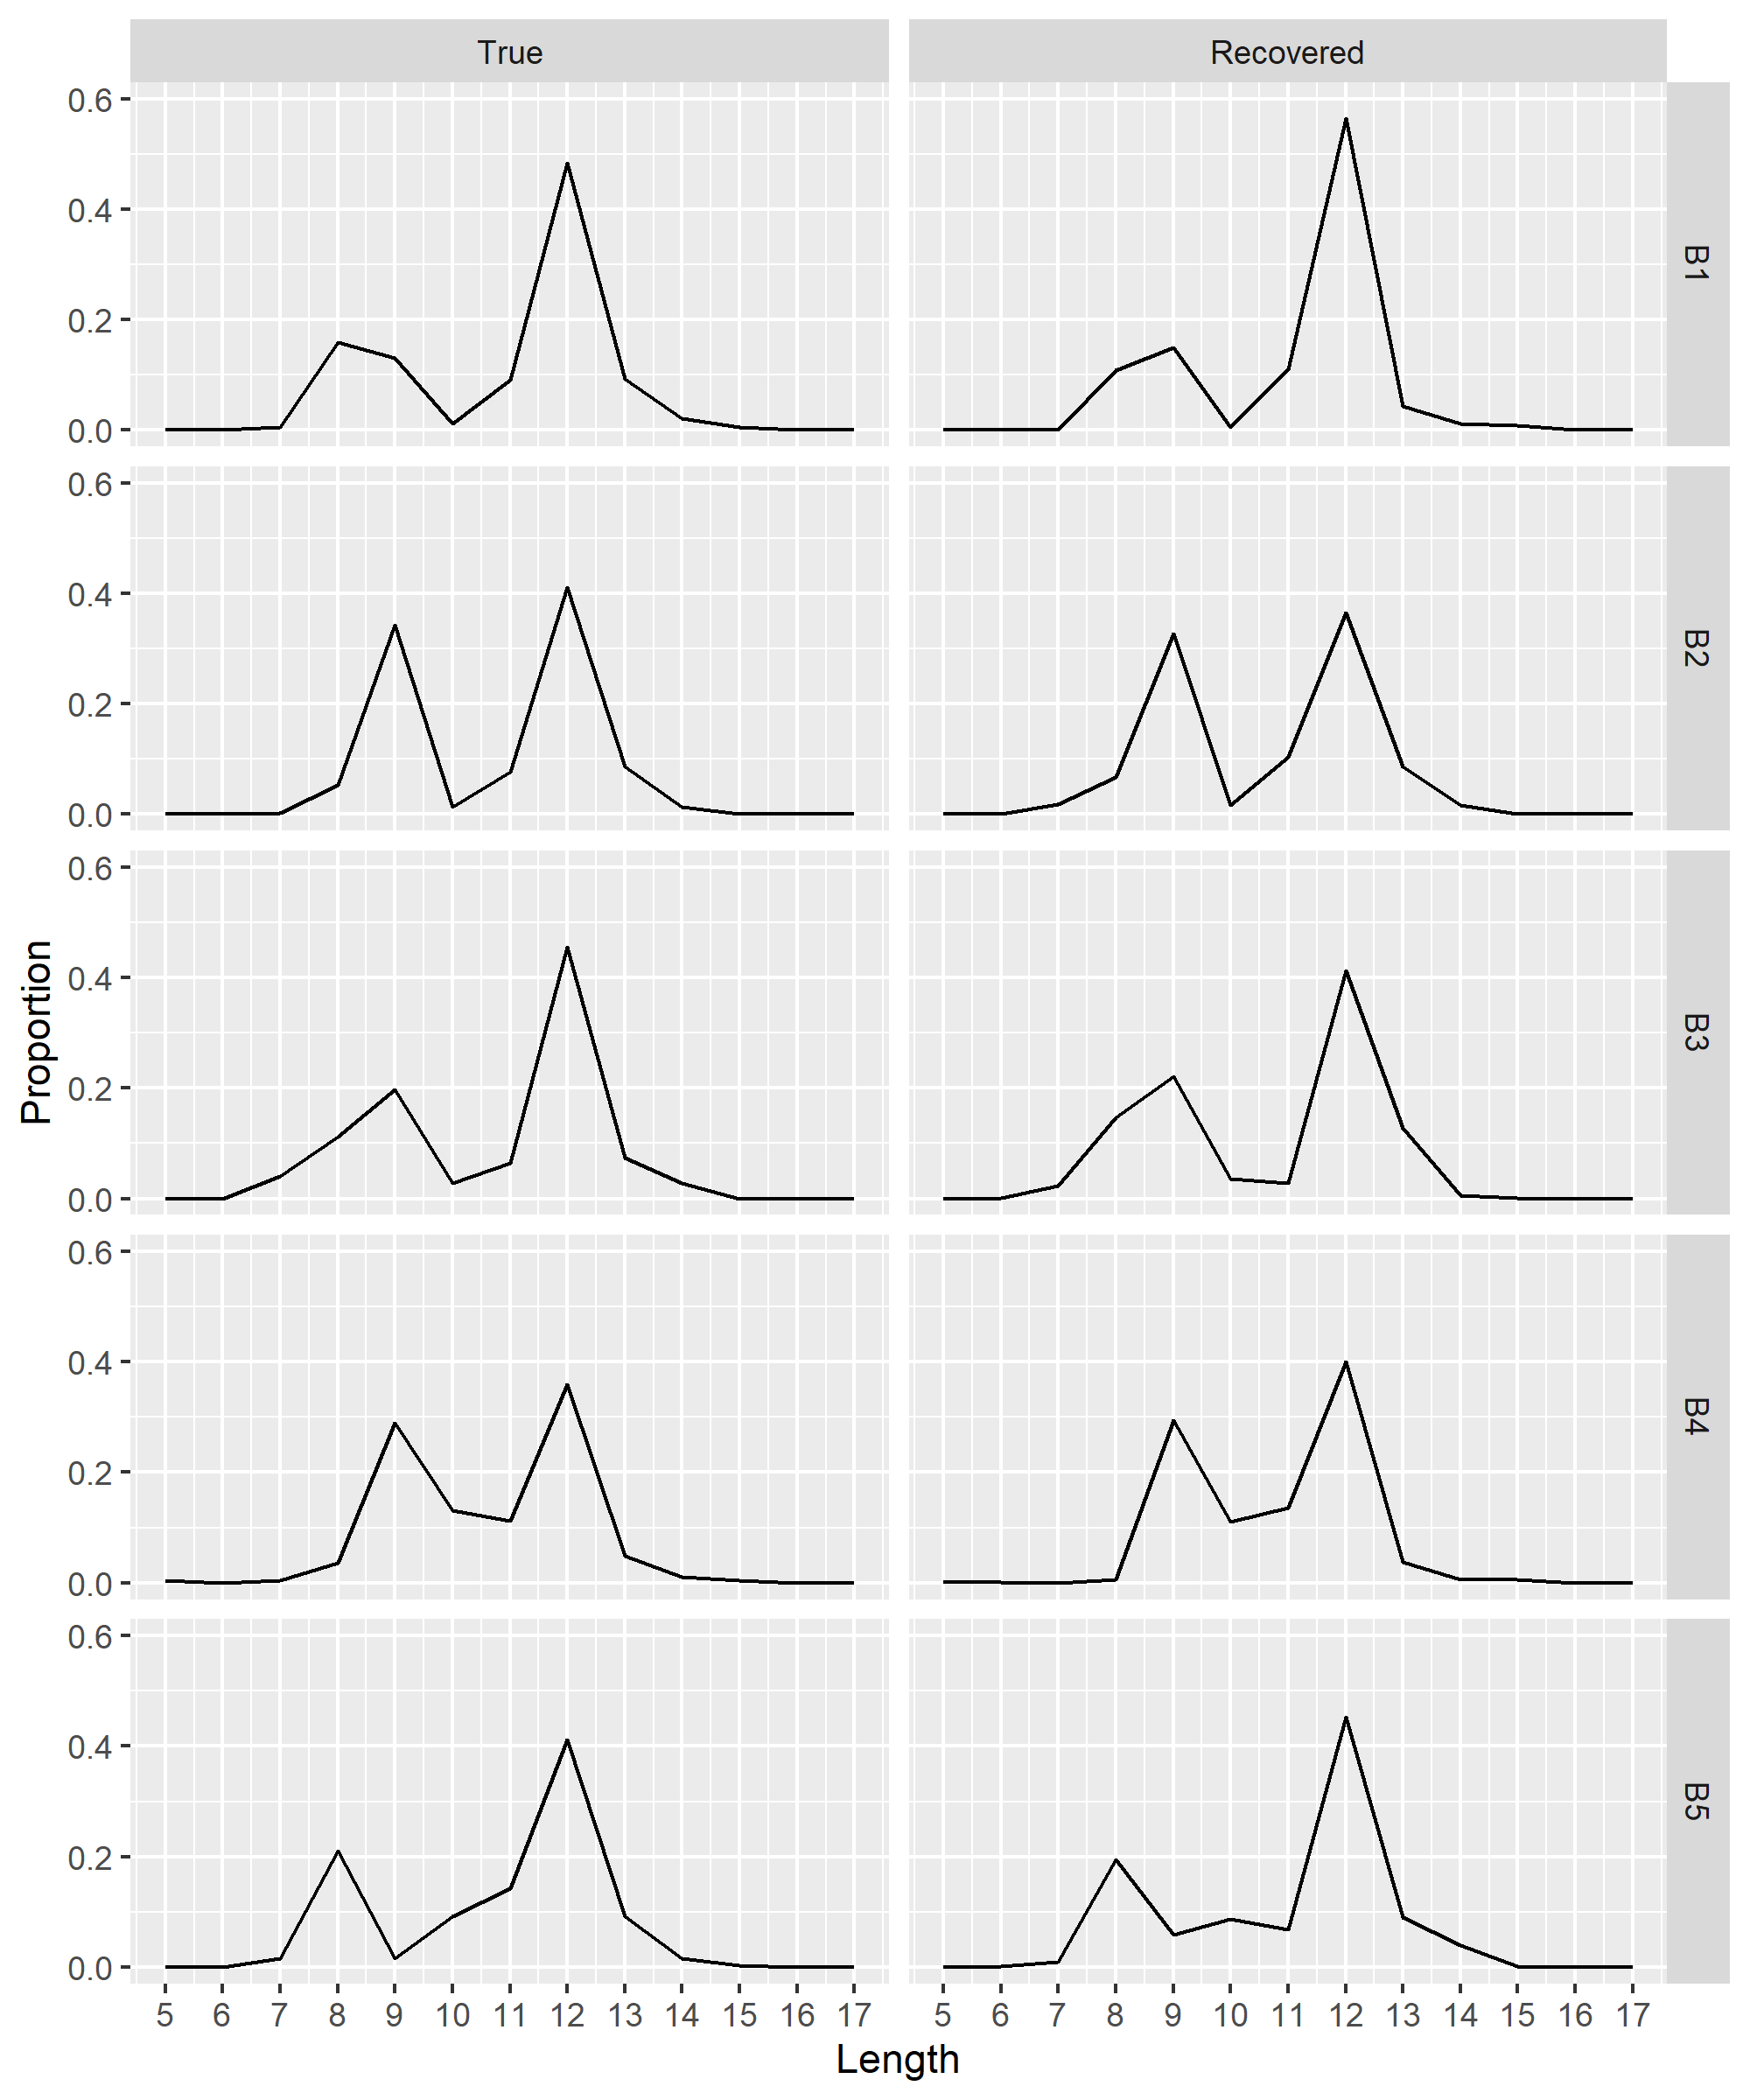
\includegraphics[width=0.8\linewidth,keepaspectratio]{images/msiclones/benchmark_loci}
	\caption[Representative microsatellite locus length distributions in benchmarking samples and recovered by subclonal microsatellite inference.]{Representative microsatellite locus (chr2:44445605--44445616) length distributions in benchmarking samples and recovered by subclonal microsatellite inference. Briefly, five MSI-H tumor samples and one MSS normal from separate patients were computationally mixed seven times in random proportions, and our subclonal microsatellite inference algorithm was utilized to recover their original microsatellite distribution. Results from one representative run (out of five) are depicted. True: microsatellite length distributions determined by MANTIS in each tumor sample B1--B5. Recovered: estimated microsatellite distributions via subclonal microsatellite inference. Proportion: estimated proportion of alleles with each microsatellite length in a sample. Length: number of bases in microsatellite locus.}
	\label{fig:msiclones:benchmark_locus}
\end{figure}

To assess the performance of the above method of subclonal microsatellite estimation, we utilized sequencing reads from five MSI-H tumors (confirmed by IHC) and a normal blood sample, each obtained from separate patients (Supplemental File~S\thechapter{}.2). These patients were sequenced with an in-house targeted clinical NGS assay, along with probes targeting 99 loci for an in-house MSI probe panel. 97 of these loci were sufficiently covered in all of these tumor samples for usage by MANTIS\@. We created five virtual patients by computationally mixing these six biological samples in varying proportions, with the normal sample providing known germline microsatellite distributions, and the five MSI-H tumors used as pure subclones. For each virtual patient, we generate a random $\mathbf{P} \in \mathbb{R}^{6 \times 7}$ matrix, corresponding to five tumor subclones and normal, along with seven tumor samples. Each column of each $\mathbf{P}$ is independently generated \cite{decamps2020} such that:
\begin{equation}
	\mathbf{P}_{*i} \sim \text{Dirichlet}(6, \vec{w}_i) \qquad i = 1 \twodots 7
\end{equation}
where each vector of concentration parameters $\vec{w}_i \in \mathbb{Z}^6$ is drawn without replacement from the set \{2, 5, 6, 7, 8, 12, 20\}.

We then create seven virtual tumor samples for each virtual patient, with normal and clonal fractions determined by $\mathbf{P}$. Define $\vec{d} \in \mathbb{Z}^6$ as the number of sequenced reads in each of the six biological samples. For each virtual tumor sample $i = 1 \twodots 7$, we first compute the maximum number of reads drawable from a biological sample while not exceeding the number of available reads in any biological sample:
\begin{equation*}
	m = \min_{k = 1 \twodots 6}\left(\frac{d_k}{P_{ki}}\right)
\end{equation*}
Finally, from each biological sample $k = 1 \twodots 6$, we include each read with a probability of $\frac{m P_{ki}}{d_k}$ in the virtual sample. These virtual samples were aligned as above (Section~\ref{ssec:msiclones:sampleseq}), and microsatellite instability and length distributions called with MANTIS (Section~\ref{ssec:msilandscape:mantis}).

We next applied our subclonal microsatellite analysis to each virtual patient, attempting to recover the microsatellite distributions of each biological sample (Figure~\ref{fig:msiclones:benchmark_locus}). For each microsatellite locus in each biological sample, we have known $f_k(l)$, the pmf of microsatellite lengths in sample $k$ for $l \in L$ microsatellite lengths in the sample, and our analysis approach generates an estimated pmf of microsatellite lengths $\hat{f}_k(l)$. Computing the Pearson correlation between $f_k(l)$ and $\hat{f}_k(l)$, along with its associated $P$ value, yields a measure of the accuracy of recovering the true microsatellite length distribution from multiple heterogeneous samples. A locus was considered as recovered in a subclone if its estimated subclonal microsatellite length distribution had a Pearson correlation with the corresponding tumor sample's microsatellite length distribution yielding $P < 0.001$ (Supplemental File~S\thechapter{}.3). Our subclonal microsatellite inference method achieved an average recovery rate of 96.2\% (s.d.\ 1.8\%). Code for microsatellite inference and benchmarking is available at Code Ocean: \url{https://codeocean.com/capsule/2769076/}.

It should be noted that this benchmarking approach provides a measure of the accuracy of our subclonal microsatellite inference method under two assumptions; that all clonal populations are identified, and that the subclonal composition of each sample (but not necessarily their phylogenetic relationship) is exactly known. Single-cell whole genome sequencing \cite{navin2011} has demonstrated that most if not all cells in a tumor have at least some genetic differences that cannot be fully modeled with any reasonable number of ``subclones'', therefore these assumptions cannot be shown to be met with current subclonal inference methodologies. At best, subclonal inference provides a biologically meaningful model of tumor evolution even though it cannot fully capture the genomic complexity of cancer. Therefore, we believe that our simulation with mixed samples provides a reasonable approximation for benchmarking our method of deconvolving subclonal microsatellite distributions, while providing ``true'' microsatellite distributions for comparison with the output of our method.

\subsection{Subclonal MANTIS-equivalent scores}
\label{ssec:msiclones:mantis_equiv_scores}
After determining per-subclone microsatellite distributions, we computed MANTIS-\linebreak{}equivalent microsatellite instability scores. Similar to the per-locus microsatellite instability scores calculated by MANTIS (Equation~\ref{eqn:msilandscape:mantis_sum}), for each locus $r$ we computed a stepwise distance between tumor and normal for each subclone $k-1 \in 2 \twodots K$:
\begin{equation}
    d_r(k) = \sum_{l \in L}|\hat{M}_{l1} - \hat{M}_{lk}|
\end{equation}
From these per-locus subclonal MANTIS scores, we also computed a MANTIS-equivalent score for each entire subclone:
\begin{equation}
    s(k) = \frac{\sum_{r \in R} d_r(k)}{|R|}
\end{equation}
Though all subclones in all patients met the MANTIS threshold for a tumor sample to be called MSI-H (0.4), it should be noted that this threshold was calibrated for MSI-H detection in a tumor tissue sample and matched normal rather than subclones. For instance, subclones are a mathematical approximation of a pure tumor cell population rather than a heterogeneous and impure tumor sample, and small microsatellite shifts can lead to substantial net differences in length distribution. Therefore, we avoid assigning MSS or MSI-H status to entire subclones solely on the basis of MANTIS scores. We classified each locus $r$ in subclone $k$ with score $d_r(k)$ as unstable if $1.0 < d_r(k) \le 2.0$ or stable if $d_r(k) \le 1.0$ (Figure~\ref{fig:msiclones:subclonal_ms_hist}). Furthermore, loci unstable in all subclones are termed ``ubiquitously unstable'', in more than one but not all subclones ``shared unstable'', in one subclone only ``private unstable'', and in no subclones ``stable''. We estimate expected values ($E$) for the number of ubiquitous, shared, private, and stable loci through simulating 1,000 random distributions of unstable loci in each subclone, and use chi-square tests to compute $P$ values. For significance of overlapping ubiquitously unstable loci across patients, $P$ values were calculated by comparison versus 10,000 random distributions of ubiquitous loci.
\begin{figure}[ht]
	\centering
	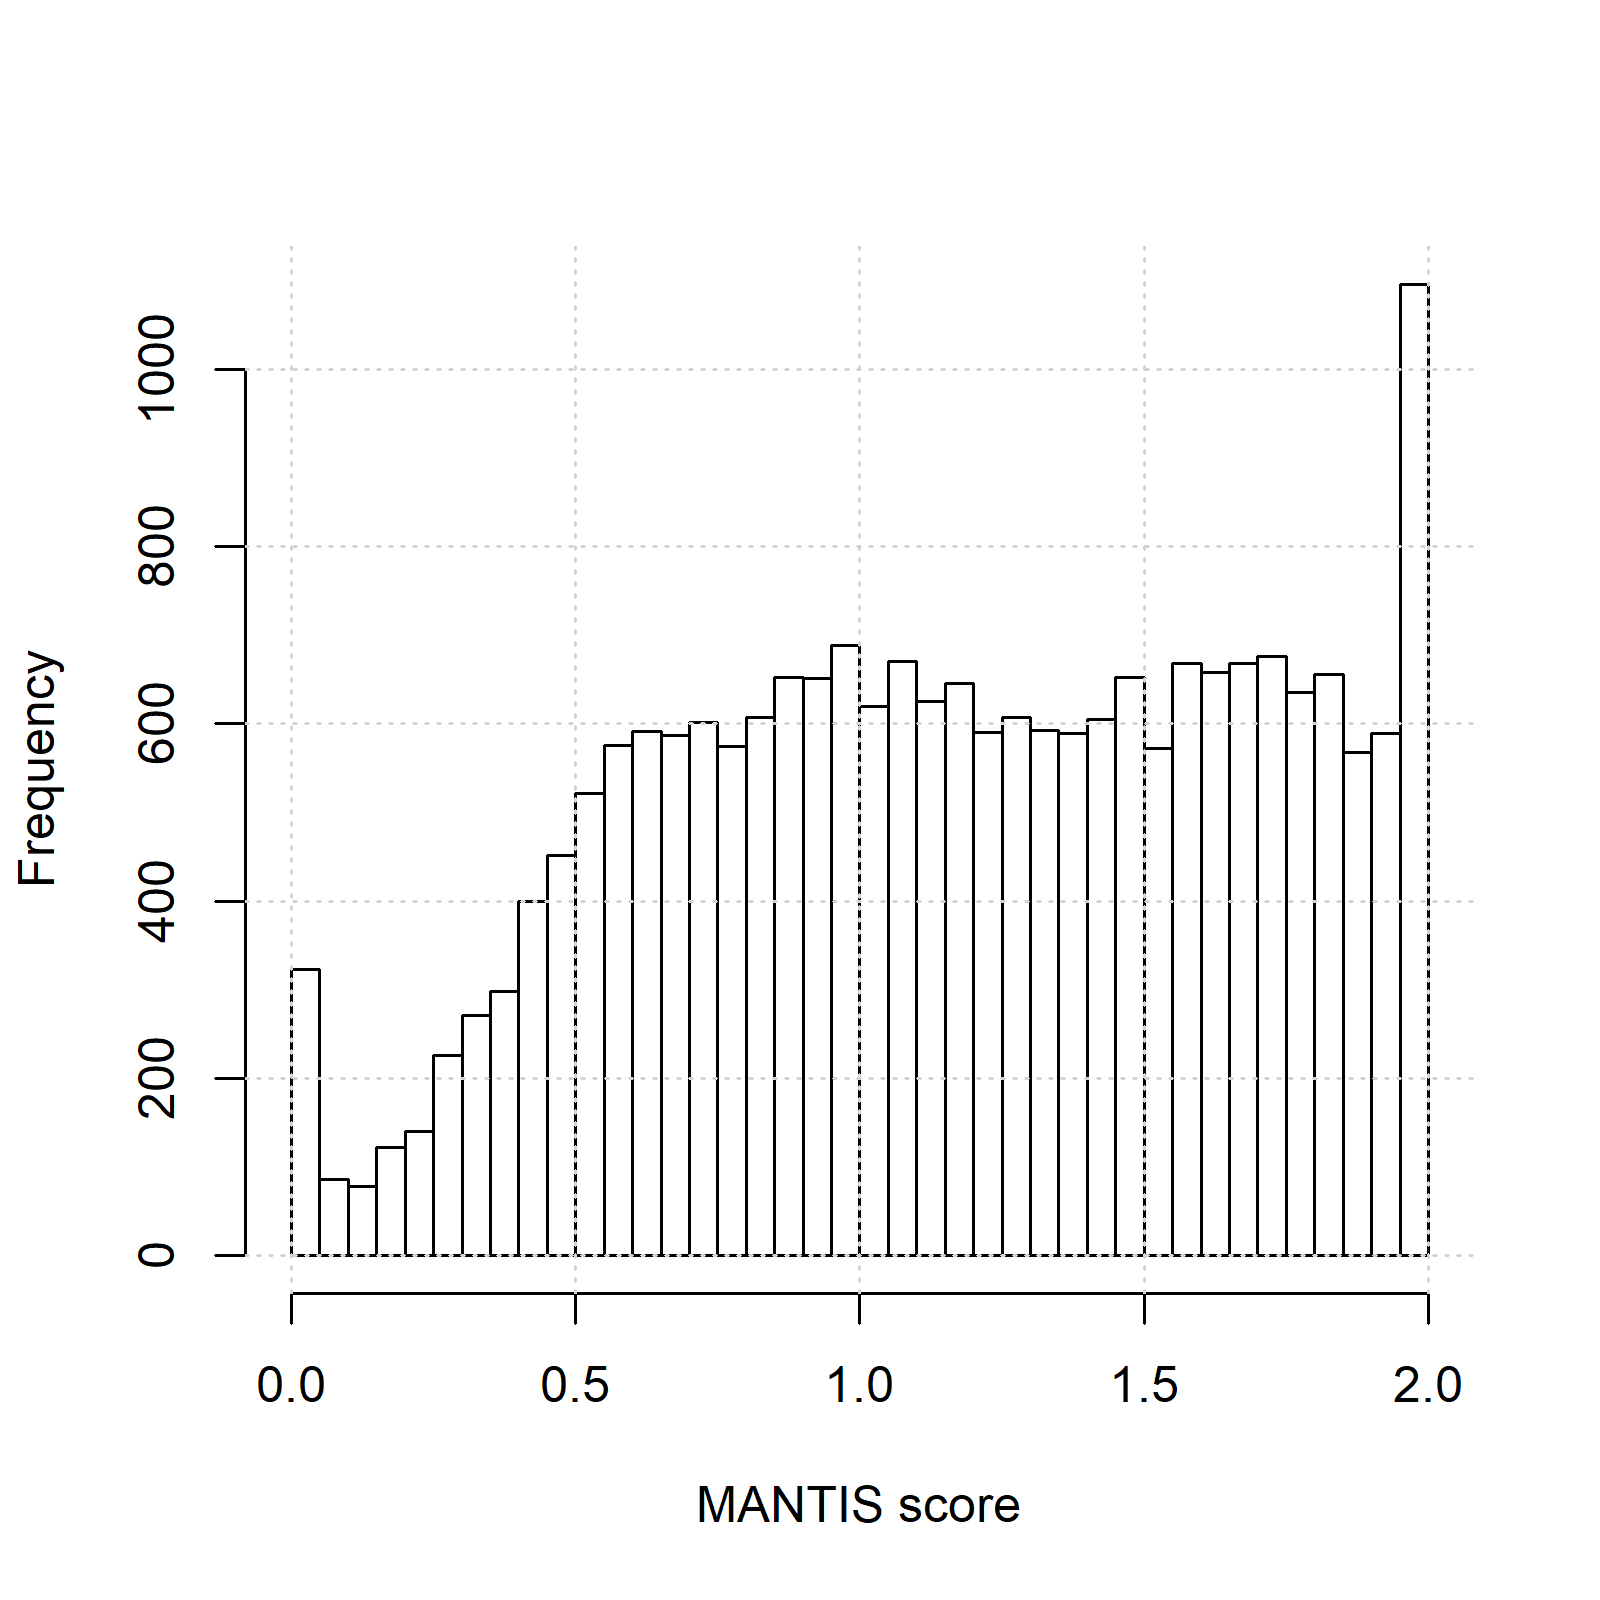
\includegraphics[width=0.7\linewidth]{images/msiclones/all_subclonal_ms_hist}
	\vspace{-0.5cm}
	\caption[Distribution of subclonal microsatellite MANTIS scores across all samples.]{Distribution of subclonal microsatellite MANTIS scores across all samples. Given the range of MANTIS scores as [0.0--2.0], and the approximate uniformity of the center of the distribution, we chose 1.0 as a threshold to classify an individual locus as microsatellite unstable on a subclonal basis.}
	\label{fig:msiclones:subclonal_ms_hist}
\end{figure}

To compute the per-subclone coverage of a locus $r \in R$ in a patient, consider $\vec{j}_r \in \mathbb{R}^N$, the total coverage of this locus in all samples. Therefore, the number of reads expected in this patient from each subclone (and from germline) is simply $\mathbf{P}\vec{j}_r$. Averaging these values for all loci used by MANTIS in a patient yields the average subclonal locus coverage, with higher coverage corresponding to increased confidence in estimated subclonal microsatellite length distributions.

To analyze shifts in microsatellite lengths, we filtered the sets of covered microsatellite loci within each patient for loci with an unambiguous single germline length. Loci with:
\begin{equation}
	\max(\hat{M}_{*1}) \ge \gamma
	\label{eqn:msiclones:gm_loci}
\end{equation}
for $\gamma = 0.7$ were selected. This yielded from 136 to 313 loci. We then computed the mean, median, mode, standard deviation and skewness of microsatellite lengths in each subclone for these loci.

We computed normalized most recent common ancestor similarities (nMRCA) as follows. Within any subclone $k \in 2 \twodots K$ within a patient, we have a set of variants $V_k$. For any pair of subclones $k_1, k_2 \in 2 \twodots K$, we have:
\begin{equation}
    \text{nMRCA}(k_1, k_2) = \frac{|V_{k1} \cap V_{k2}|}{\max_{k \in 1 \twodots K} |V_k|}
    \label{eqn:msiclones:nmrca}
\end{equation}
We computed the Pearson correlation coefficient between $d(k_1)$ and $d(k_2)$ of per-locus stepwise differences, and utilized linear regression of these correlations versus \mbox{nMRCA} to quantify the relationship between common clonal ancestry and similarity of microsatellite instability.

The statistical significance of this regression was computed via a bootstrapping scheme. We generated 1,000 random $\mathbf{P}$ matrices for each of the six patients with the same dimensions as the original matrices, and applied our simulated annealing approach to estimate subclonal microsatellite distributions. For computational considerations, only one chain was run for 10,000 iterations for each set of matrices. Regression between nMRCA and pairwise microsatellite distance correlation was performed as above to generate a set of correlations under this random null.

\subsection{Alternative subclonal inference}
For all six patients, subclonal inference was performed with SuperFreq \cite{flensburg2020} as well as Canopy. Aligned sequencing reads were filtered using SAMtools to exclude multiple-mapped reads and any reads aligning outside the exome and CNV capture regions. Preliminary single-sample variant calling was performed with GATK version 4.0.10, with minimum base quality score 30, 2 maximum alternate alleles at a site, and soft-clipped bases ignored. SuperFreq version 1.3.2 was then run using R version 3.5.0, with systematic variance of 1.0 (to mitigate noisy CNV calls) and all other parameters left at default. For each patient, all tumor samples were run against the panel of normals from all six patients.

As SuperFreq frequently calls clones at very low fractions, we enforced a minimum clonal fraction of 5\% for any subclone in any sample, below which the clonal fraction is set to zero. For a phylogeny $G = (V, E)$, with the root node $v_1$ corresponding to germline and other nodes for tumor subclones, accompanied by clonal fraction matrix $\mathbf{P} \in \mathbb{R}^{|V| \times N}$, we apply:
\begin{algorithm}[H]
	\caption{Minimal SuperFreq clonal fraction}
	\label{alg:msiclones:min-clonal-frac}
	\begin{algorithmic}[1]
		\Procedure{MinimalFraction}{$G, v, \mathbf{P}$}
			\ForAll{$w$ s.t. $(v, w) \in E$}
				\State $\mathbf{P}_{v*} \gets \mathbf{P}_{v*} +$ \Call{MinimalFraction}{$G, w, \mathbf{P}$}
			\EndFor
			\State $\vec{r} \gets$ all elements of $\mathbf{P}_{v*} < 0.05$, which then $\gets 0$ if $v \neq v_1$
			\State \textbf{return} $\vec{r}$
		\EndProcedure
		\State \Call{MinimalFraction}{$G, v_1, \mathbf{P}$}
	\end{algorithmic}
\end{algorithm}

SuperFreq typically delineates many more subclones than Canopy for the same input samples. As the number of subclones tends to exceed the number of samples, we were unable to apply our subclonal microsatellite inference algorithm to these clonal decompositions as this would yield underdetermed systems of equations (Section~\ref{ssec:msiclones:subclonal_msi}). Although this could be overcome through distributional assumptions reducing the number of parameters to estimate, we chose to avoid \textit{a priori} assumptions of a specific distribution as no previous studies have investigated microsatellites within subclones and germline microsatellite lengths often follow bimodal distributions due to differing lengths inherited from each parent.

\section{Results}
\subsection{Clinical histories}
\label{ssec:msiclones:clinical_histories}
\begin{figure}[p]
	\begin{center}
		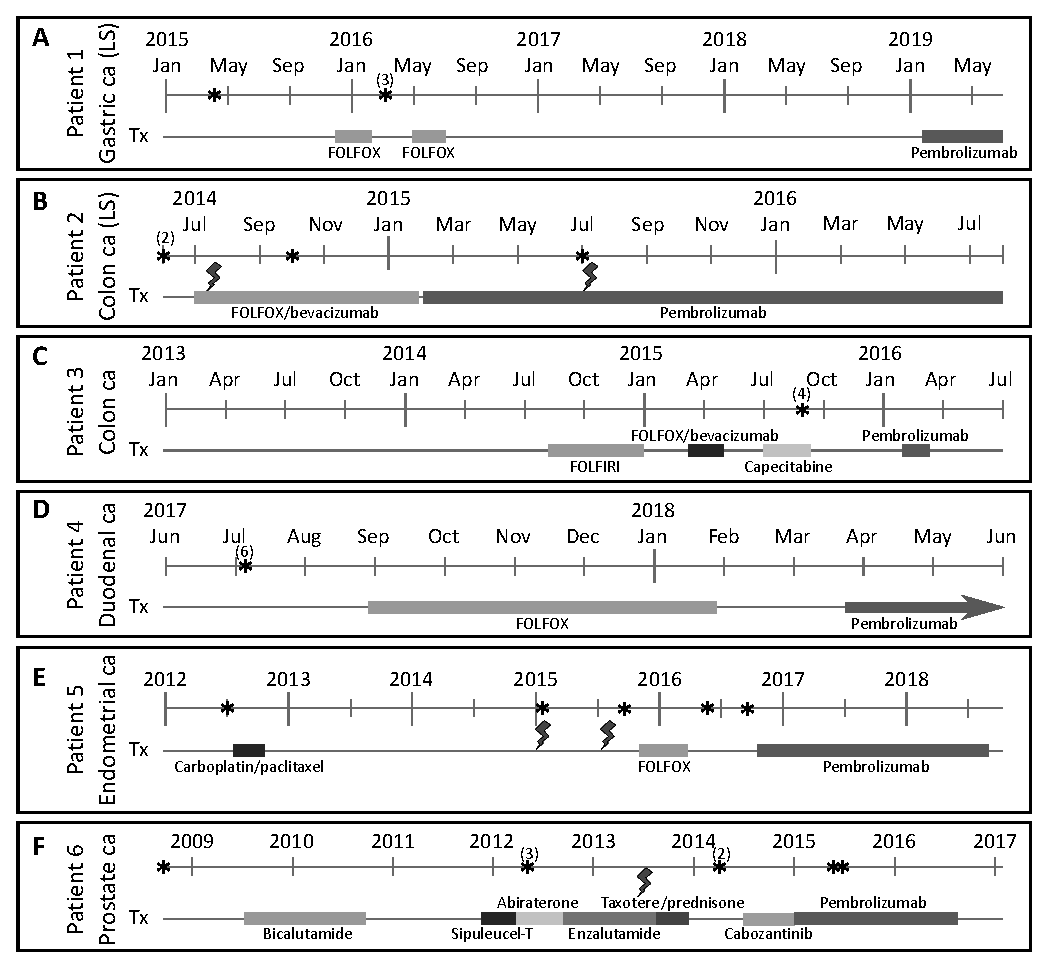
\includegraphics[width=0.94\linewidth]{images/msiclones/clinical_timelines}
	\end{center}
	\vspace{-0.4cm}
	\caption[Clinical courses of six patients with MSI-H metastatic cancers.]{Clinical courses of six patients with MSI-H metastatic cancers. \textbf{(a)}: 53-year old female with gastric cancer. \textbf{(b)}: 31-year old female with colon cancer. \textbf{(c)}: 77-year old female with colon cancer. \textbf{(d)}: 67-year old male with duodenal cancer. \textbf{(e)}: 63-year old female with endometrial cancer. \textbf{(f)}: 85-year old male with prostate cancer. Shaded boxes represent the duration of each treatment modality. Asterisks delineate time points when samples were acquired, and numbers in parentheses indicate acquisition of multiple samples from the same time point. Lightning symbols denote radiotherapy. FOLFOX: folinic acid, 5\nobreakdash-fluorouracil, oxaliplatin. FOLFIRI: folinic acid, 5\nobreakdash-fluorouracil, irinotecan. LS: Lynch syndrome.}
	\label{fig:msiclones:clinical_hx}
\end{figure}
Patient 1 is a 53-year old female with previously known Lynch syndrome (Figure~\ref{fig:msiclones:clinical_hx}a). A colonoscopy in January 2015 revealed colon cancer, and she underwent a right hemicolectomy and prophylactic total hysterectomy with bilateral salpingoophorectomy (TAH/BSO) in April 2015. A polyp was identified containing moderately differentiated adenocarcinoma with mucinous features, and MSH2/MSH6 negative by immunohistochemistry (IHC)\@. An enteroscopy in December 2015 identified gastric cancer, and she received neoadjuvant 5\nobreakdash-fluorouracil, folinic acid, and oxaliplatin (FOLFOX) from December 2015 to February 2016. She underwent total gastrectomy along with excision of the greater omentum and proximal lymph nodes in March, which identified moderately differentiated adenocarcinoma with mucinous and pyloric gland features that was MSH2/MSH6 negative by IHC\@. She then received adjuvant FOLFOX from May to July 2016, then elected for surveillance. Lung metastases were detected in November 2018, and she began pembrolizumab in February 2019. She continued on pembrolizumab until she developed acute thyroiditis in July 2019. She remains off treatment with stable disease in her lungs as of October 2019.

Patient 2 is a 31-year old female with known Lynch syndrome who first presented in May 2014 with bloody stools, unplanned weight loss, nausea\slash{}vomiting, and influenza-like symptoms (Figure~\ref{fig:msiclones:clinical_hx}b). Radiologic imaging indicated a 7~cm proximal colon mass, along with metastases to the liver, right adrenal gland, right kidney, pericecal lymph nodes, and upper paraaortic lymph nodes. She underwent a right hemicolectomy in June, which revealed poorly differentiated adenocarcinoma that was MSI-H by PCR (5/5 unstable markers) and MLH1/PMS2 negative by IHC\@. Next, she received FOLFOX\slash{}bevacizumab. In July, she presented with a destructive right femur bone lesion, which required radiation therapy. After FOLFOX\slash{}bevacizumab treatment, follow-up imaging indicated shrinkage of liver and lung metastases and stabilization of the bone metastasis. She continued on FOLFOX\slash{}bevacizumab until January 2015, when she developed gastrointestinal bleeding. In February 2015, she began a clinical trial (OSU-14006) for pembrolizumab in MSI-H solid tumors. Subsequent imaging in July showed a metastasis in the vermis of the cerebellum but no other evidence of disease. She underwent surgical resection of this cerebellar lesion followed by radiation treatment. Repeat imaging indicated no evidence of cancer, and she continued on pembrolizumab until November 2016, when it was stopped due to autoimmune side effects. She remains off treatment and in complete remission as of August 2019.

Patient 3 is a 77-year old female, who was initially diagnosed in 2013 with colon cancer and underwent transverse colon resection in April (Figure~\ref{fig:msiclones:clinical_hx}c). She was found to have abdominal recurrence in July 2014, which was treated with combination 5\nobreakdash-fluorouracil, folinic acid, and irinotecan (FOLFIRI) beginning in August. FOLFIRI was stopped in January 2015 due to disease progression, and she received combination chemotherapy with FOLFOX\slash{}bevacizumab from March to May, followed by capecitabine monotherapy from July to September. Due to worsening obstructive symptoms suggestive of clinical progression, she underwent resection of her abdominal tumor, small bowel, and a partial colectomy in September 2015. Her tumor was found to be MSH2/MSH6 absent by IHC, and negative for p63, CK5/6, chromogranin, and synaptophysin. She was enrolled in OSU-14006 and received two pembrolizumab infusions in February and March 2016, however treatment was discontinued in April due to infusion reactions. She remains off treatment with stable disease as of January 2020.

Patient 4 is a 67-year old male who presented in June 2017 with clay-colored stool, unplanned weight loss, jaundice, and early satiety (Figure~\ref{fig:msiclones:clinical_hx}d). Imaging indicated acute pancreatitis and a mass between the pancreatic head and duodenum. He underwent a Whipple procedure and right hemicolectomy in July, which revealed duodenal adenocarcinoma, positive for CK7, CK20, CDX2, CAM5.2 and vimentin, and negative for PAX-8. MSI-PCR indicated MSI-H with 5/5 unstable loci. He received adjuvant FOLFOX from August 2017 to January 2018. Imaging in March 2018 identified recurrence in his liver along with retroperitoneal adenopathy. He began pembrolizumab, which was continued until February 2020.

Patient 5 is a 63-year old female with a history of ductal carcinoma in situ (DCIS) of the breast, which was treated with radiation and tamoxifen (Figure~\ref{fig:msiclones:clinical_hx}e). In April 2012, she underwent TAH/BSO for vaginal bleeding, which revealed stage 1B poorly differentiated endometrioid adenocarcinoma, positive for CK7 and negative for CK20, ER, PR, \mbox{PAX-8} and mammaglobin. This was followed by four cycles of adjuvant chemotherapy with carboplatin\slash{}paclitaxel until September 2012. In January 2015 she was found to have a right femur metastasis, and a biopsy revealed moderate-poorly differentiated adenocarcinoma of unknown primary, positive for AE1/3, CK7, \mbox{CDX-2}, \mbox{GATA-3}, mucin and vimentin, and negative for CK20, \mbox{TTF-1}, ER, PR and \mbox{PAX}-8. She underwent a prophylactic right femur nailing followed by radiation to the surgical site. She was also found to have an epigastric subcutaneous soft tissue mass. In June, she received radiotherapy for a right calvarial bone metastasis. Imaging in September 2015 indicated progression in her abdominal soft tissue metastasis, and she began FOLFOX chemotherapy in October. She continued on FOLFOX until February 2016, with stable disease. She developed bowel obstructive symptoms and weight loss, and underwent a bowel resection in May 2016. Her tumor was found to be MSH2/MSH6 negative by IHC, and MSI-PCR indicated MSI-H with 5/5 unstable loci. She began pembrolizumab in August 2016 and achieved a complete response to therapy. She completed two years of therapy in July 2018, and currently remains off treatment and under surveillance as of August 2019.

Patient 6 is an 85-year old male who presented in December 2008 with high-risk prostate cancer (Figure~\ref{fig:msiclones:clinical_hx}f). He underwent a radical prostatectomy, and his tumor was graded as Gleason 5+3 and staged as T3bN1. Shortly after surgery in June 2009, his prostate specific antigen (PSA) was rising, and he began bicalutamide with good PSA response (decrease). In September 2010, his PSA rebounded, prompting bicalutamide withdrawal. He began dietary intervention with soy\slash{}almond supplements, which ended in May 2011 and achieved a PSA decline. However, his PSA increased again in December 2011, and restaging scans indicated progressive disease with periumbilical lymphadenopathy and a new nodule at his bladder. Sipuleucel-T (Provenge\textsuperscript{\textregistered{}}) was initiated, but shortly after new imaging revealed a large (\textgreater{}~10~cm) abdominal tumor involving the adjacent bowel requiring surgery. He subsequently received abiraterone\slash{}prednisone and enzalutamide, but his disease continued to progress. In October 2013, he was switched to taxotere\slash{}prednisone, which was stopped in December due to continued progression. He underwent a radical resection of an abdominal tumor in February 2014, which was found to be MSH2/MSH6 negative by IHC\@. He began cabozantinib in May 2014. This was discontinued in December 2014 due to disease progression. He began pembrolizumab in January 2015, and underwent two cystoscopies one week apart with transurethral resection of his bladder tumor in April and May 2015. Treatment was stopped August 2016 due to complete response, and he remains in remission, off treatment, and under surveillance as of August 2019.

\subsection[WES demonstrates mismatch repair-deficient hypermutation]{Whole exome sequencing demonstrates mismatch repair-\linebreak{}deficient hypermutation}
\begin{figure}[ht]
	\begin{center}
		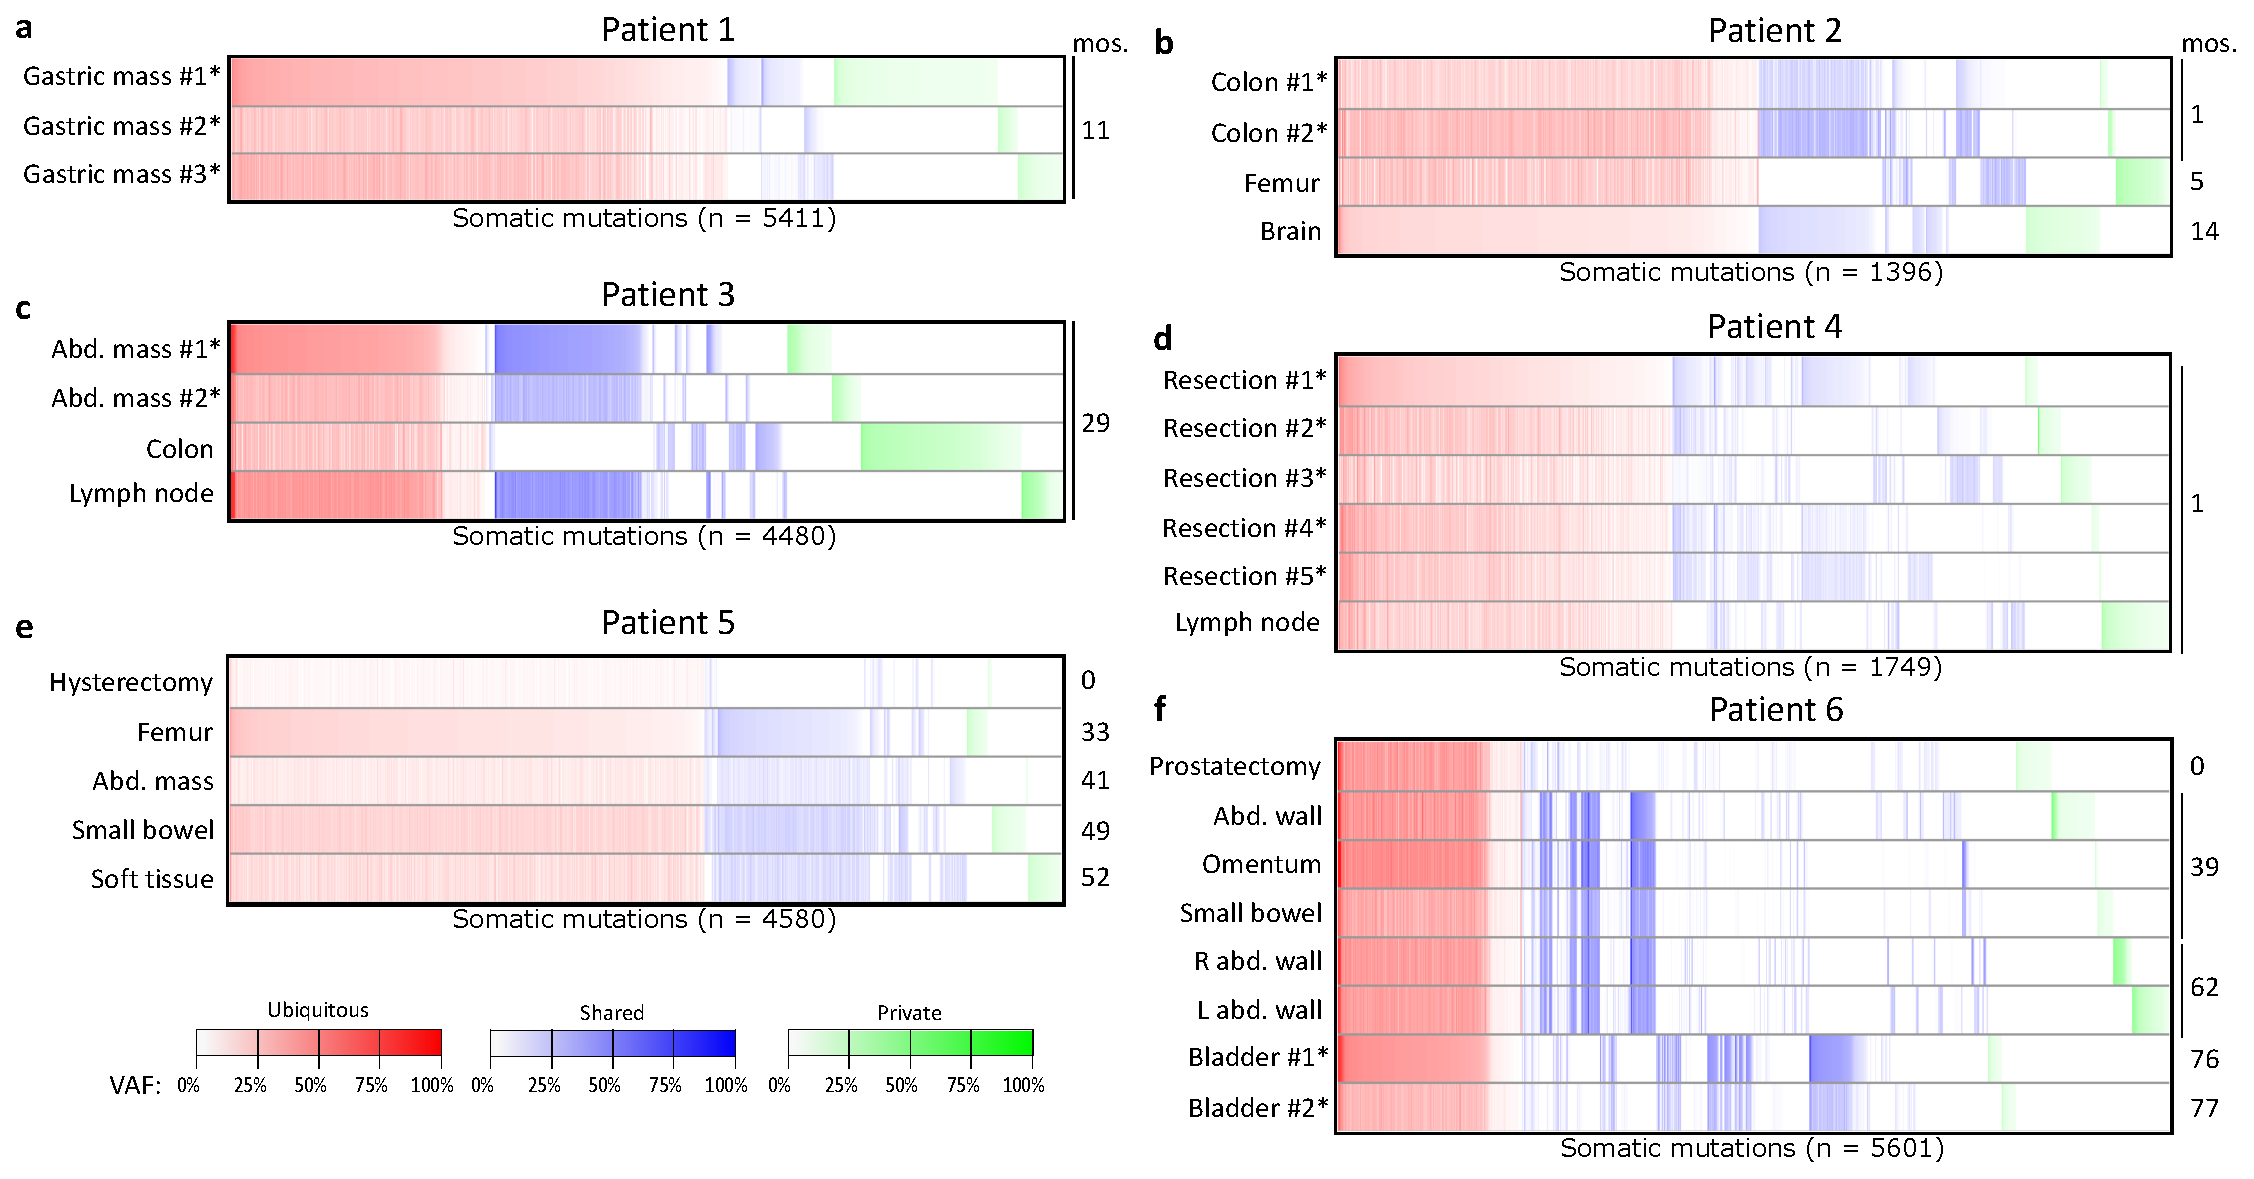
\includegraphics[width=0.98\linewidth]{images/msiclones/mutations_by_sample_min0}
	\end{center}
	\vspace{-0.4cm}
	\caption[Somatic mutations (SNVs and indels) called in at least one tumor sample.]{Somatic mutations (SNVs and indels) called in at least one tumor sample from six patients with MSI-H cancers \textbf{(a--f)}. The colon polyp sample from patient 1 was excluded due to suspicion of arising from a separate primary tumor than the gastric mass samples. Note that in patient 6, bladder \#1 and bladder \#2 were acquired from separate surgeries one week apart. Within each heatmap, columns in red represent mutations with at least one alternate-supporting read in all tumor samples (whether or not the variant was called in all samples), columns in blue represent mutations with alternate-supporting reads in one but not all tumor samples, and columns in green represent mutations with alternate-supporting reads in only one tumor sample. Samples marked with asterisks were acquired from a single tumor mass in that patient. mos: months post-diagnosis. Abd: abdominal. VAF: variant allele fraction.}
	\label{fig:msiclones:mutation_heatmaps}
\end{figure}

We performed whole exome sequencing on 31 tumor samples and six matched normal blood samples from six patients (average coverage 218\texttimes{}, Supplemental File~S\thechapter{}.2) with MSI-H metastatic cancers. Except for the hysterectomy sample from patient 5, all tumor samples were hypermutated (Figure~\ref{fig:msiclones:mutation_heatmaps}), with an average tumor mutational burden (TMB) of 53.0~mutations/Mb in patient 1, 23.0 in patient 2, 58.1 in patient 3, 19.7 in patient 4, 79.3 in patient 5, and 47.7 in patient 6. There were 1,396 to 5,601 total unique mutations (SNVs and indels) with a minimum variant allele fraction (VAF) of 6\% detected in each patient (Figure~\ref{fig:msiclones:mutation_heatmaps_min0}, Supplemental File~S\thechapter{}.4). Except for the patient 5 hysterectomy sample, all samples were estimated to contain at least 30\% tumor cells. We also identified six discrete CNVs in patient 6 (Supplemental File~S\thechapter{}.4). None of the other patients had CNVs passing thresholds.

All samples from each patient were called MSI-H by MANTIS (Supplemental File~S\thechapter{}.1) and bore mutational signatures characteristic of MMRd-induced hypermutation (any of signatures 6, 15, 20, and 26) (Supplemental File~S\thechapter{}.4). Patients 1--4 and 6 possessed signature 6 in all samples, and all patient 5 samples contained signature 20. Patient 5 was also notable for signature 14, which in conjunction with signature 20 is associated with combined polymerase proofreading and MMRd \cite{haradhvala2018}. We identified mutations in MMR genes in five of six patients. Patients 1 and 2 had the germline mutations \textit{MSH2} p.Q493X and \textit{MLH1} p.K618del respectively. All patient 3 and 5 samples contained MMR stop-gain mutations (\textit{MLH1} p.Q346X and \textit{MSH2} p.Q324X, respectively), and a region of chromosome 2p containing \textit{MSH6} was deleted in all samples from patient 6. For patient 4, an epigenetic modification such as \textit{MLH1} hypermethylation is a likely possibility, however IHC was not available to identify specific MMR protein loss. In addition, a \textit{POLD1} p.E318K mutation was found in three samples from patient 5.

\begin{table}[H]
    \begin{center}
    	\begin{tabular}{r:ccc}
    		Patient & Ubiquitous & Shared & Private \\
    		\hline
    		1 & 15 & 2036 & 3360 \\
    		2 & 552 & 300 & 544 \\
    		3 & 982 & 1055 & 2443 \\
    		4 & 364 & 527 & 858 \\
    		5 & 74 & 3423 & 1083 \\
    		6 & 991 & 1392 & 3218
    	\end{tabular}
	\end{center}
	\vspace{-0.3cm}
	\caption[Ubiquitous, shared, and private mutations identified across patient tumor samples.]{Numbers of ubiquitous, shared, and private mutations identified across tumor samples from patients 1--6. Ubiquitous mutations are defined as detected in all tumor samples from a patient, shared mutations as detected in more than one but not all tumor samples, and private mutations as detected in only one sample.}
	\label{table:msiclones:ubiq_shared_priv_muts}
\end{table}

Next, we assessed the overlap of mutations among tumor samples within each patient (Figure~\ref{fig:msiclones:mutation_heatmaps}, Table~\ref{table:msiclones:ubiq_shared_priv_muts}). Groupings of mutations were observed by organ sites, for instance among the patient 2 colon samples and patient 6 abdominal vs.\ bladder samples. Fewer than 40\% of mutations were ubiquitous (present in all tumor samples with at least 6\% VAF) in any patient (Figure~\ref{fig:msiclones:mutation_heatmaps_min0}), which suggests the presence of substantial heterogeneity among these tumors. Patients 1 and 5 had very low proportions of ubiquitous mutations, instead containing an abundance of private (present in one tumor sample) and shared (neither ubiquitous nor private) mutations. Within patient 1, the colon polyp sample contained almost exclusively private mutations, with only 50 of its 2,407 mutations (2.1\%) found in any of the three gastric mass samples. In contrast, the three gastric masses were genetically more similar, with 1,489 of the 5,411 total mutations (27.5\%) in this patient present in every gastric sample. Of the 2,836 mutations called in at least one gastric mass sample but not the colon polyp, only 42 (1.5\%) had at least five alternate-supporting reads in the colon polyp. As 47 (1.7\%) of those mutations had at least five alternate-supporting reads in patient 1's abdominal mass, and in conjunction with the neighbor-joining tree of these samples (Figure~\ref{fig:msiclones:NJ_trees_1}), the colon polyp likely represents a separate primary and was therefore excluded from further analysis, which focuses on her gastric cancer. In patient 5, 4,283 of the 4,580 total mutations were not called in the hysterectomy sample at 6\% VAF\@. This is most likely due to its low tumor purity, as 1,179 of these 4,283 mutations (27.5\%) had at least five alternate-supporting reads in the hysterectomy sample (Figure~\ref{fig:msiclones:mutation_heatmaps}). Based on this substantial overlap, we conclude that the 2015 and 2016 samples represent recurrence of the 2012 endometrial cancer, contrary to the clinical diagnosis of separate primaries.

\begin{figure}[htp]
	\centering
	\begin{subfigure}{0.49\textwidth}
		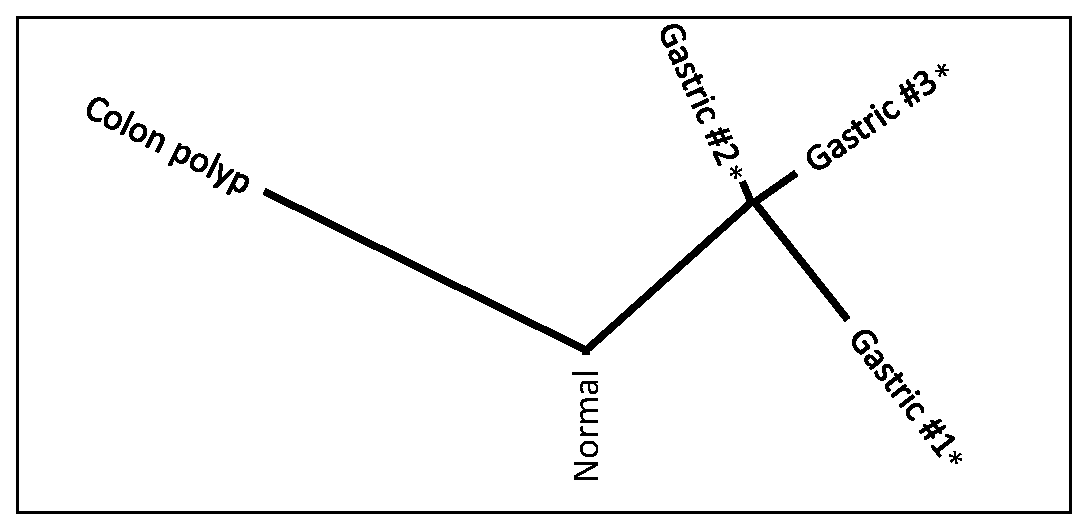
\includegraphics[width=\linewidth,keepaspectratio]{images/msiclones/supp_nj_1}
		\caption{}\label{fig:msiclones:NJ_trees_1}
	\end{subfigure}%
	\hfill%
	\begin{subfigure}{0.49\textwidth}
		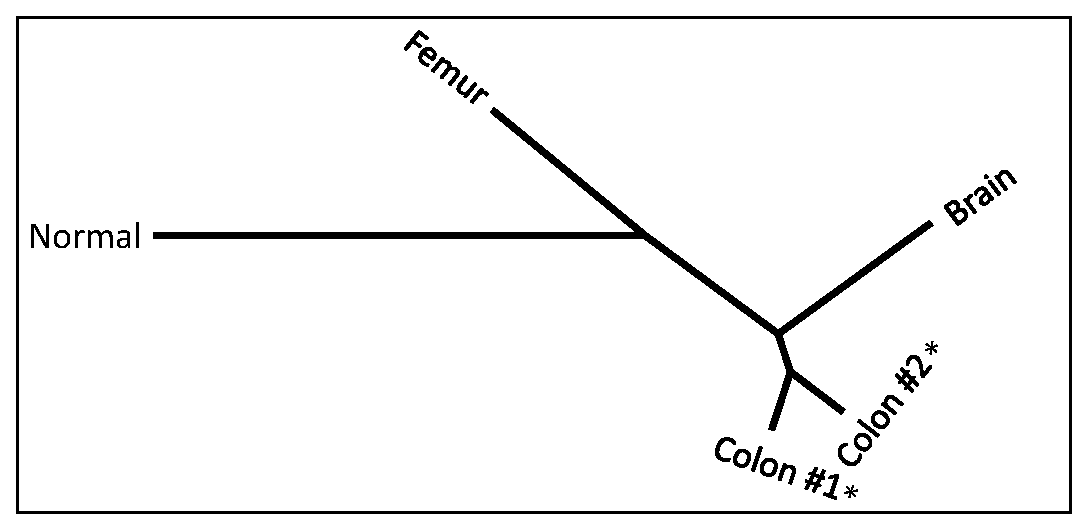
\includegraphics[width=\linewidth,keepaspectratio]{images/msiclones/supp_nj_2}
		\caption{}\label{fig:msiclones:NJ_trees_2}
	\end{subfigure}
	\par
	\begin{subfigure}{0.49\textwidth}
		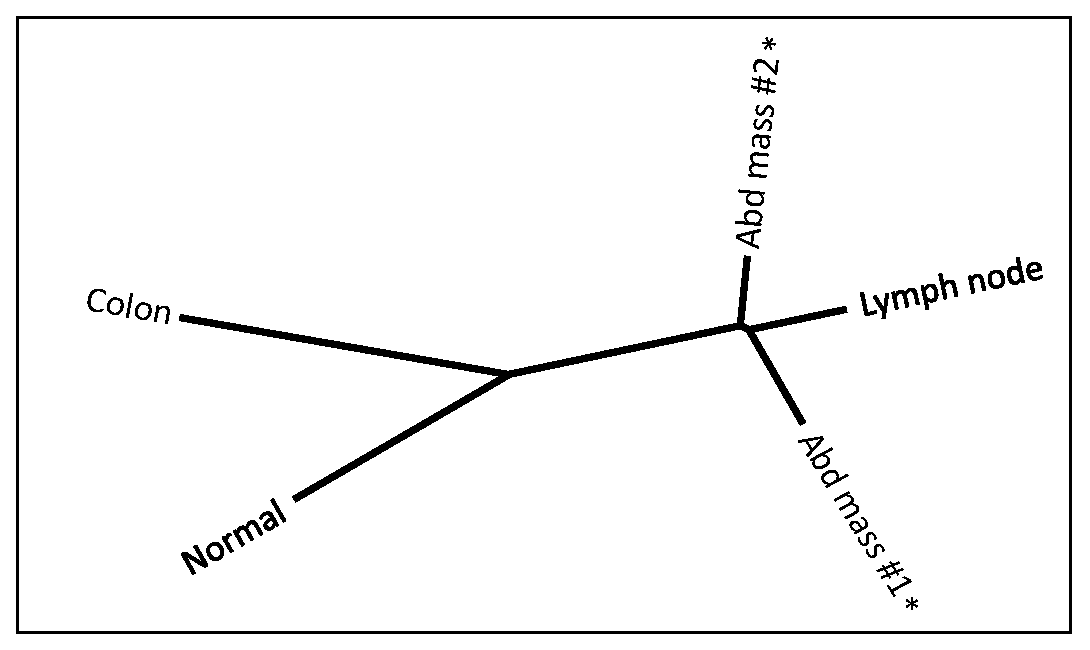
\includegraphics[width=\linewidth,keepaspectratio]{images/msiclones/supp_nj_3}
		\caption{}\label{fig:msiclones:NJ_trees_3}
	\end{subfigure}%
	\hfill%
	\begin{subfigure}{0.49\textwidth}
		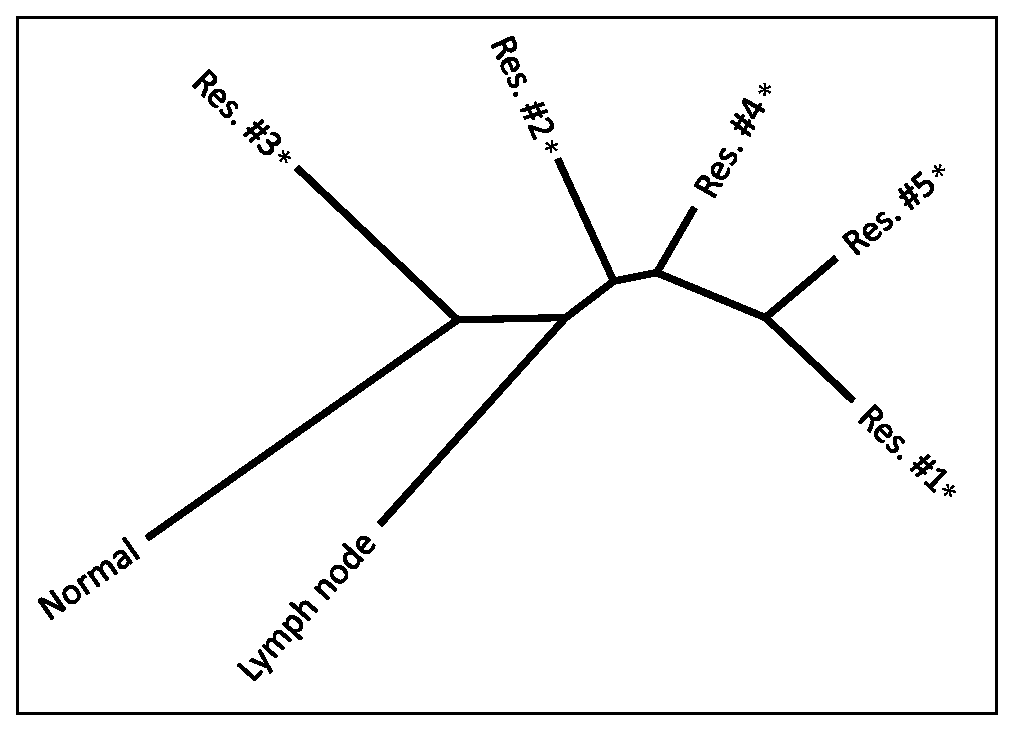
\includegraphics[width=\linewidth,keepaspectratio]{images/msiclones/supp_nj_4}
		\caption{}\label{fig:msiclones:NJ_trees_4}
	\end{subfigure}
	\par
	\begin{subfigure}{0.49\textwidth}
		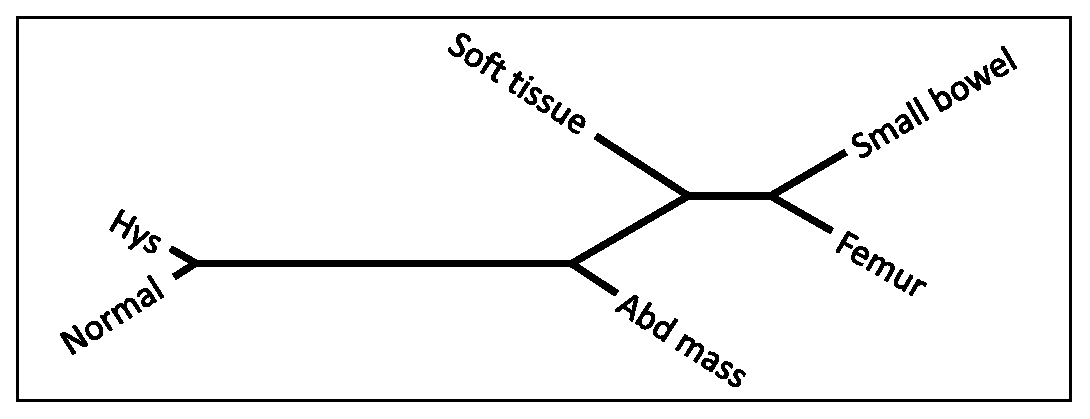
\includegraphics[width=\linewidth,keepaspectratio]{images/msiclones/supp_nj_5}
		\caption{}\label{fig:msiclones:NJ_trees_5}
	\end{subfigure}%
	\hfill%
	\begin{subfigure}{0.49\textwidth}
		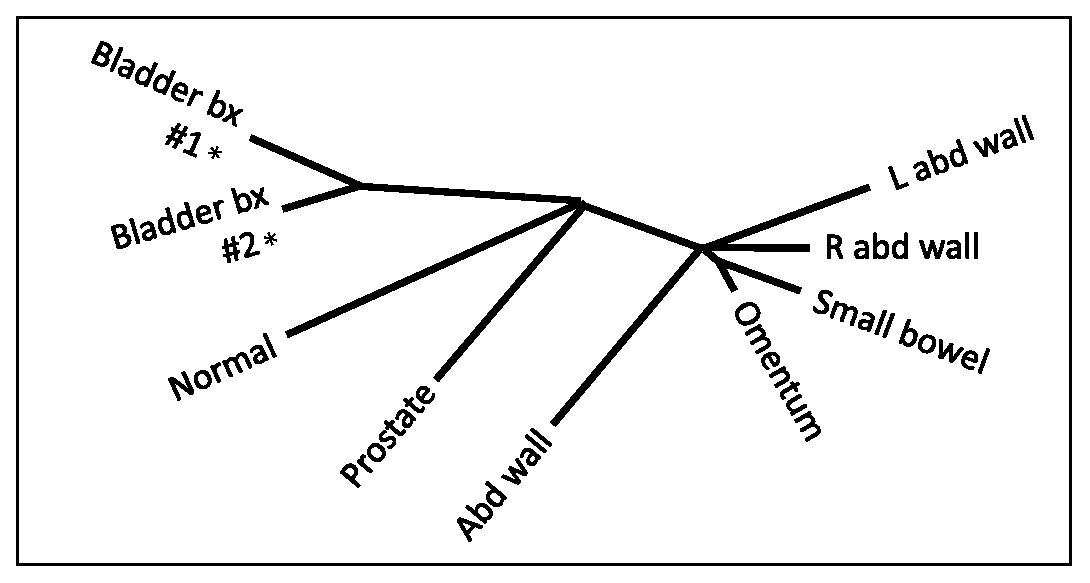
\includegraphics[width=\linewidth,keepaspectratio]{images/msiclones/supp_nj_6}
		\caption{}\label{fig:msiclones:NJ_trees_6}
	\end{subfigure}
	\caption[Neighbor-joining (NJ) trees of genetic relatedness between tumor samples.]{Neighbor-joining (NJ) trees of genetic relatedness between tumor samples from (\subref{fig:msiclones:NJ_trees_1}) patient 1, (\subref{fig:msiclones:NJ_trees_2}) patient 2, (\subref{fig:msiclones:NJ_trees_3}) patient 3, (\subref{fig:msiclones:NJ_trees_4}) patient 4, (\subref{fig:msiclones:NJ_trees_5}) patient 5, and (\subref{fig:msiclones:NJ_trees_6}) patient 6. NJ trees were generated over a Hamming distance matrix between SNVs present in each sample using RapidNJ\@. Samples marked with asterisks were acquired from a single tumor mass in that patient. Note that in patient 6, bladder \#1 and bladder \#2 were acquired from separate surgeries one week apart. Abd: abdominal. Res: resection. Hys: hysterectomy.}
	\label{fig:msiclones:NJ_trees}
\end{figure}

We applied neighbor joining to samples in each patient as an initial survey of genetic similarity across samples, and found relationships corresponding to both sample time points and anatomical locations (Figure~\ref{fig:msiclones:NJ_trees}). Patient 1 was notable for the colon polyp developing from essentially a different lineage than the three gastric samples, consistent with her colon and gastric cancers arising from separate primary tumors. For patient 2, the two colon samples were most similar to each other as expected. The femur sample was most similar to germline, and the brain sample most distant. In patient 3, abdominal samples grouped with the lymph node, with the colon sample more distantly related. Patient 4 was notable for the genetic diversity present among the five abdominal resection samples, implying substantial intratumor heterogeneity. Within patient 5, the hysterectomy mass was much more similar to germline than any tumor, most likely due to low tumor purity limiting the sensitivity of SNV detection. In patient 6, the prostatectomy was a relatively early outlier, as expected since it was the earliest sample acquired. Both bladder biopsies were similar to each other, and the five abdominal samples (abdominal wall, small bowel and omentum) formed a loose cluster.

\subsection{Quantification and phylogenetic classification of tumor subclones}
\label{ssec:msiclones:clone_results}
\begin{figure}[ht]
	\begin{center}
		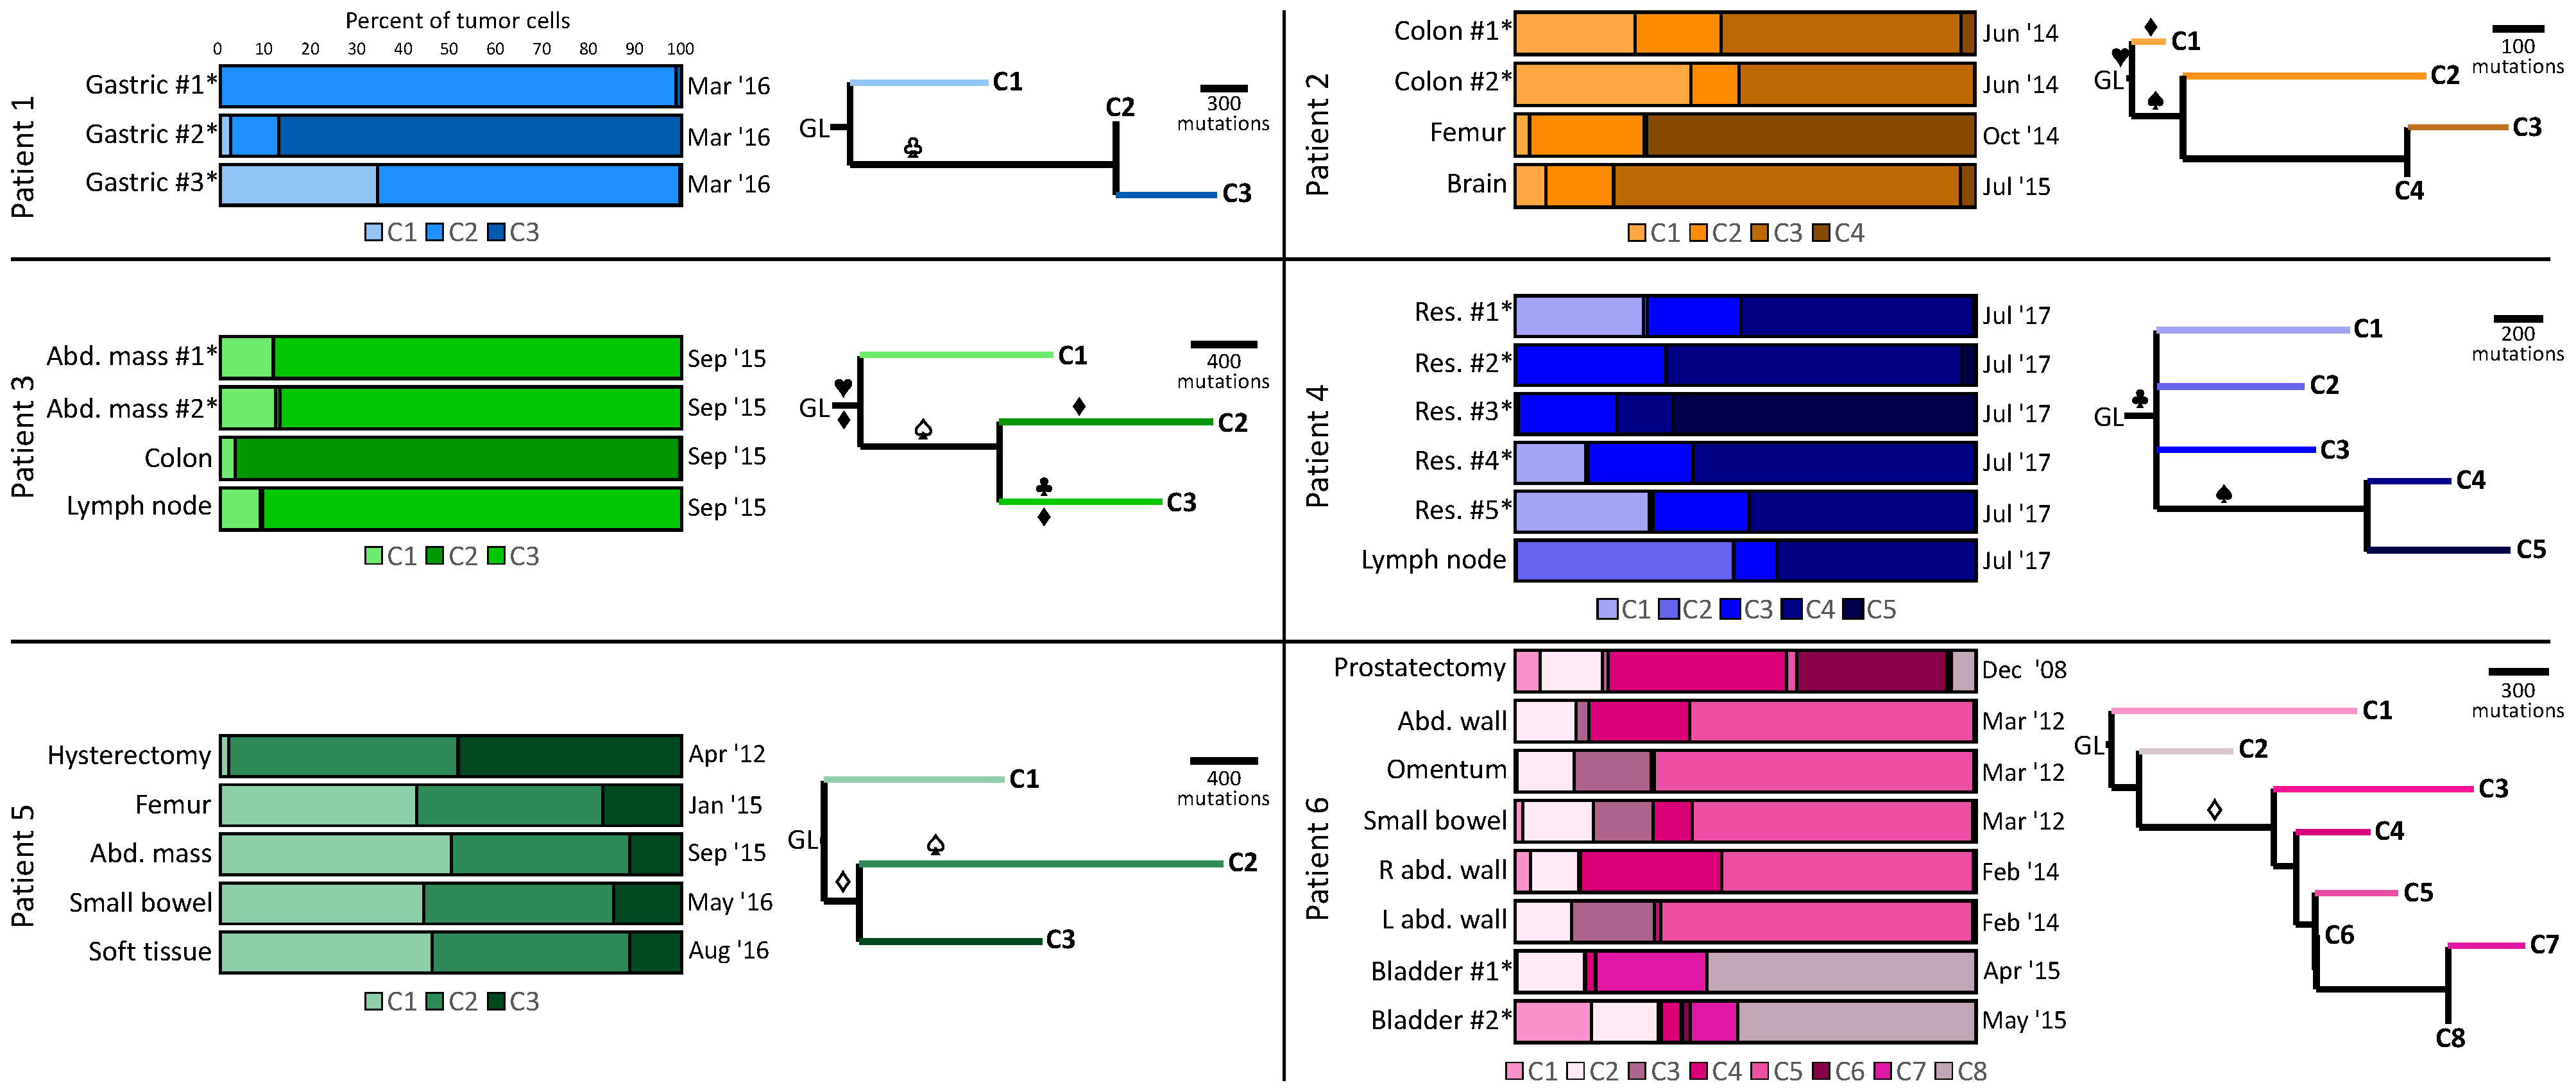
\includegraphics[width=0.98\linewidth]{images/msiclones/canopy_results}
	\end{center}
	\vspace{-0.3cm}
	\caption[Fractions of tumor subclones and estimated subclonal phylogenetic trees within six patients with MSI-H cancers.]{Fractions of tumor subclones and estimated subclonal phylogenetic trees inferred by Canopy within six patients with MSI-H cancers. Three subclones were identified in patients 1, 3 and 5, four in patient 2, five in patient 4, and eight in patient 6. Listed fractions represent the estimated proportion of tumor cells in each sample derived from each subclone. Sample acquisition dates are listed above. For patients 1--4, sequentially numbered samples were obtained from the same surgeries. Note that in patient 6, bladder \#1 and bladder \#2 were acquired from separate surgeries one week apart. For each tree, horizontal distance corresponds with increased number of mutations. Samples marked with asterisks were acquired from a single tumor mass in that patient. Symbols on the tree correspond to mutations present in a branch, with unfilled symbols indicating potentially ambiguous mutation positions based on relative statistical likelihood of assignment to other branches, and filled symbols indicating more certain position. $\blacklozenge$: MMR gene (\textit{MLH1}, \textit{MSH2}, \textit{MSH6}, or \textit{PMS2}). {\large \ETX}: \textit{CTNNB1}. $\spadesuit$: \textit{KRAS}\@. $\clubsuit$: \textit{TP53}. Res: resection. Abd: abdominal. GL: germline.}
	\label{fig:msiclones:clonal_fracs}
\end{figure}

%mention superfreq also used to check canopy, also gives opportunity to address short trunks and truncal MMR
We applied Canopy \cite{canopy}, \textit{post hoc} tree assignment of mutations, and relative mutational ordering (Section~\ref{ssec:msiclones:inference}) within each patient to identify tumor subclones and determine their phylogeny (Figure~\ref{fig:msiclones:clonal_fracs}, Supplemental File~S\thechapter{}.5), along with SuperFreq \cite{flensburg2020} as an alternate method. For brevity, we refer to Canopy subclones in patients as P\#C\#; \textit{e.g.}\ P2C3 refers to patient 2 subclone 3. Varying numbers of subclones were identified by Canopy in these six patients, from three subclones in patients 1, 3 and 5, to eight subclones in patient 6. Intratumor heterogeneity was particularly pronounced in patients 2, 4, 5 and 6, while samples in patients 1 and 3 tended to consist of pure subclones (with the exception of patient 1 gastric mass \#3). In contrast, some level of intertumor heterogeneity was evident in all patients. At least one clonally distinct sample was present in each patient, for instance subclones P1C1, P1C3, P2C4, P3C2, P4C5, and P6C6 were only prominent in one sample each, and patient 5's hysterectomy sample uniquely lacked P5C1. In addition, P2C2, P3C1, P4C3, and P6C2 were found at low levels in all samples from these patients. Consistent with the presence of substantial clonal diversity, SuperFreq identified three to sixteen clones in each patient (Figure~\ref{fig:msiclones:sf_results}, Supplemental File~S\thechapter{}.6).

\begin{figure}[ht]
	\centering
	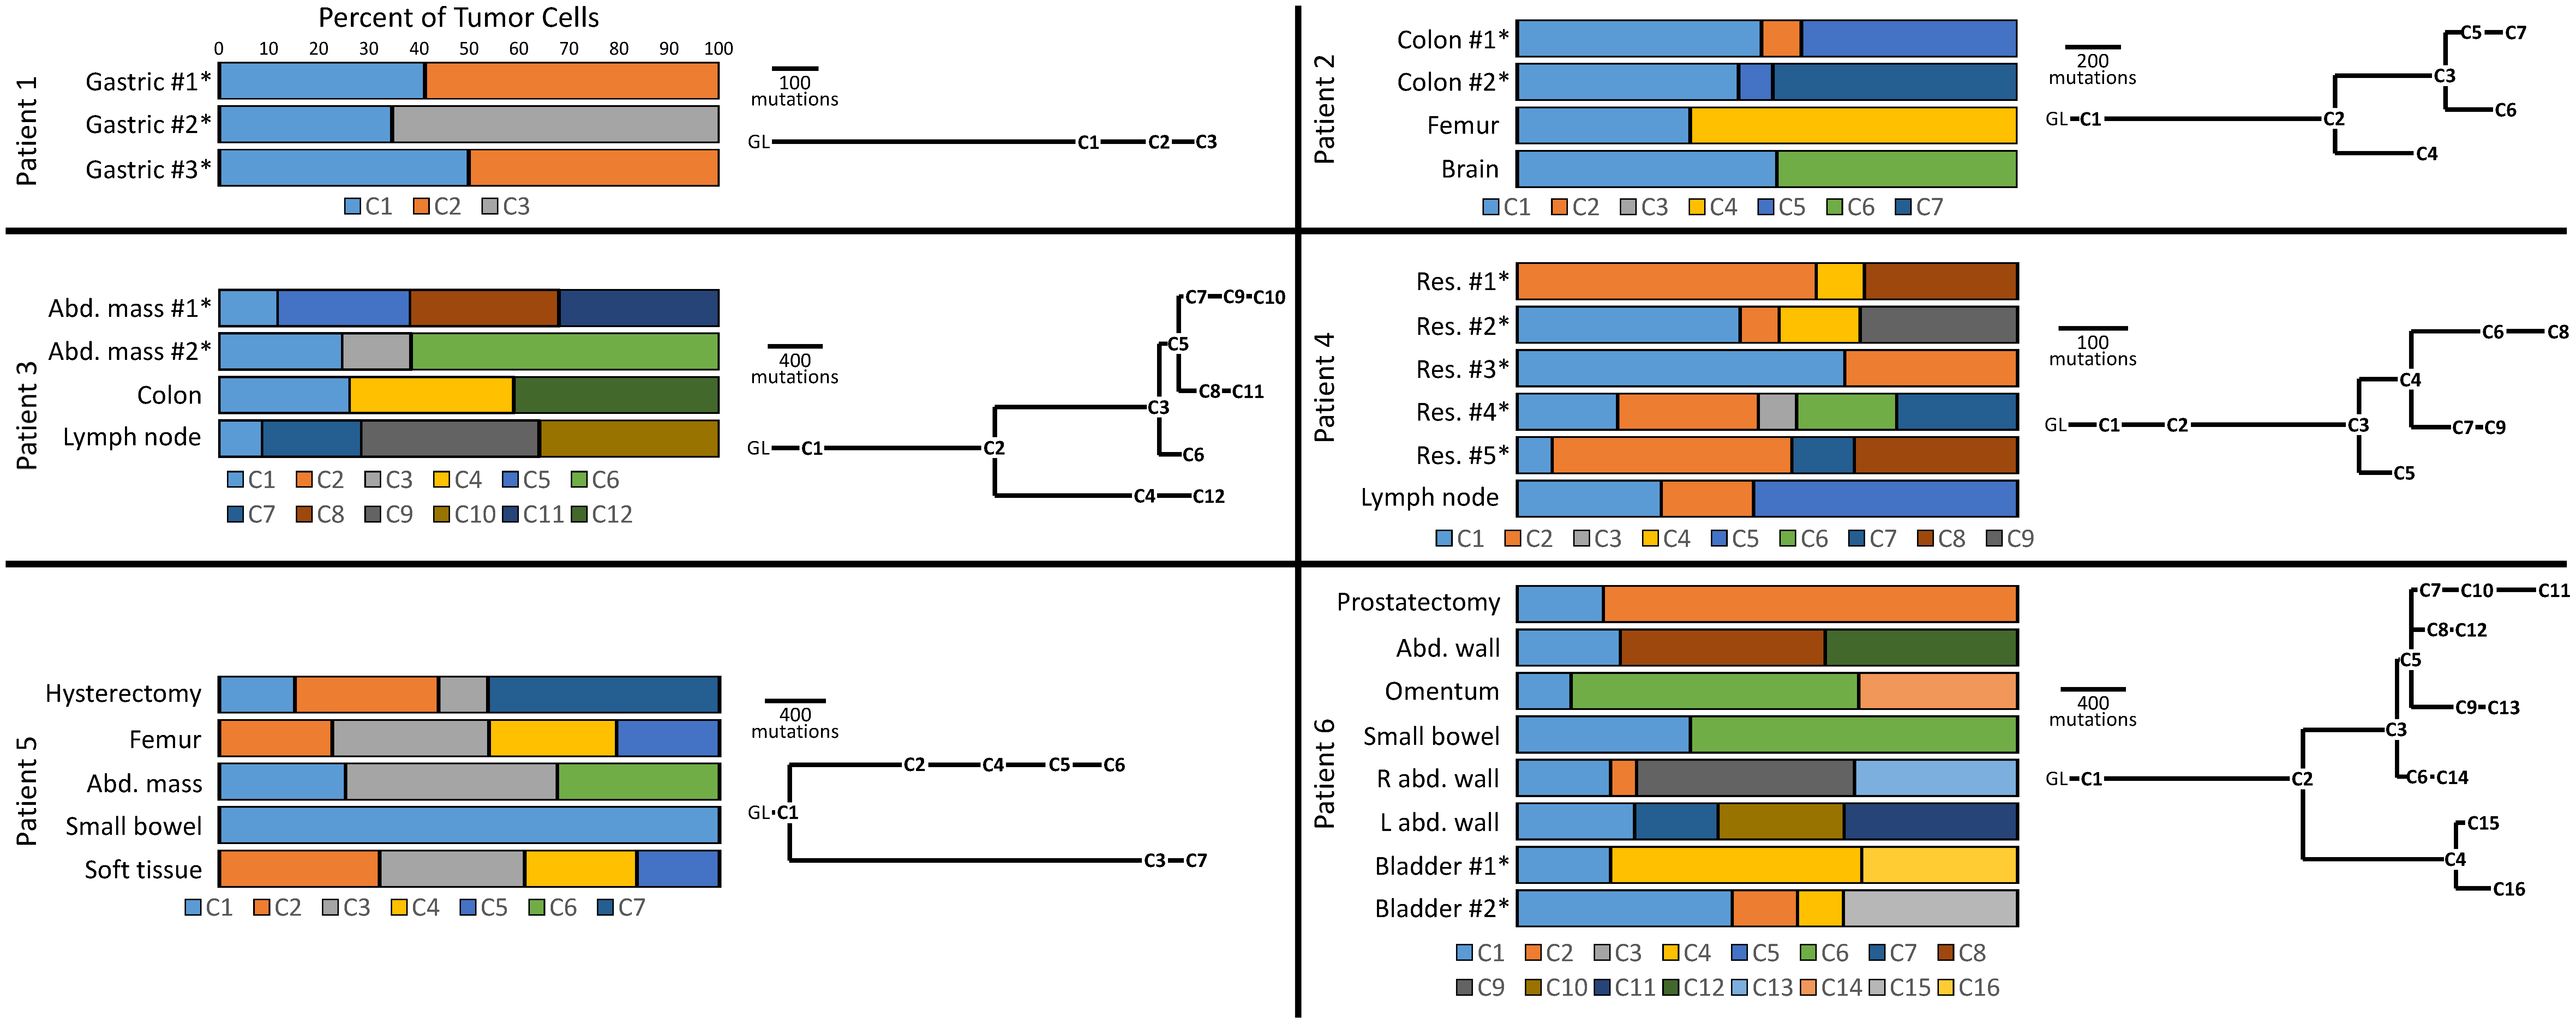
\includegraphics[width=\textwidth,height=0.83\textheight,keepaspectratio]{images/msiclones/sf_results_combined}
	\caption[Alternative subclonal inference using SuperFreq.]{Alternative analysis of subclonal evolution in patients 1--6, obtained utilizing SuperFreq rather than Canopy. Shown are estimated fractions of tumor subclones in each patient and corresponding subclonal phylogenetic trees. Three subclones were identified in patient 1, seven in patient 2, twelve in patient 3, nine in patient 4, seven in patient 5, and sixteen in patient 6. Listed fractions represent the estimated proportion of tumor cells in each sample derived from each subclone. Horizontal distance corresponds to increased number of mutations. Samples marked with asterisks were acquired from a single tumor mass in that patient. Note that in patient 6, bladder \#1 and bladder \#2 were acquired from separate surgeries one week apart. Abd: abdominal. Res: resection. GL: germline.}
	\label{fig:msiclones:sf_results}
\end{figure}

Patients 5 and 6 demonstrated clonal shifts with time. P5C1 was essentially absent in the hysterectomy sample, and emerged in the recurrent tumors sampled in 2015 and 2016. In patient 6, P6C6 was only present in the earliest sample (prostatectomy, from 2008), and absent at all later time points. The prostatectomy contained substantial P6C4 as well, which was also seen in abdominal wall samples from 2012 and 2014, but not in either 2015 sample. P6C5 was predominant in all of the 2012 and 2014 samples from the abdomen, and P6C3 was seen in two 2012 samples (omentum and small bowel) and one 2014 sample (left abdominal wall). P6C8 was predominant in both 2015 bladder samples, which also uniquely contained P6C7.

All of the phylogenetic trees inferred by Canopy for these six patients were notable for very short trunks (Figure~\ref{fig:msiclones:clonal_fracs}) containing less than 4\% of mutations (Supplemental File~S\thechapter{}.6). Short trunks were also found by SuperFreq, with less than 12\% of mutations truncal in all patients except patient 1 (Figure~\ref{fig:msiclones:sf_results}). Despite these short trunks, potentially driver truncal mutations were identified in five patients. Patients 2 and 3 had truncal \textit{CTNNB1} mutations (p.T41A and p.S45F respectively), both known driver mutations in colorectal cancer \cite{anwar2016,morin1997} known to block $\beta$-catenin ubiquitination and degradation \cite{gao2014}. Patient 4 harbored a truncal \textit{TP53} p.R273C mutation. Patient 1 possessed a \textit{TP53} p.R175H mutation in clones 2--3, however its log-likelihood of assignment to the trunk was similar, suggesting it may have been a truncal driver mutation misplaced by Canopy. The truncal branch of patient 6 was notable for \textit{LYST} p.P3167S, predicted as damaging by DANN with a score of 0.999 \cite{quang2015}. \textit{LYST} mutations are known to cause Ch\'ediak-Higashi syndrome, a pediatric condition which leads to a fatal leukemia-like accelerated phase, and have been previously described as likely drivers in chordoma \cite{tarpey2017}. We were unable to identify a potential driver mechanism among the seven nonsynonymous and exonic truncal mutations observed in patient 5.

Known and candidate pathogenic mutations were also found in specific subclones, most notably \textit{KRAS} p.G12D in P2C2--C4 and P5C2, p.G13D in P3C2--C3, and p.G12V in P4C4--C5. However, the \textit{KRAS} assignments in patients 3 and 5 were ambiguous due to similar log-likelihoods, leaving open the possibility that this is a truncal driver mutation. This likely occurred because of P3C1's low prevalence in all samples, and the poor hysterectomy tumor purity along with low intertumor heterogeneity among the other patient 5 samples. Other notable mutations included \textit{FBXW7} p.R385H, \textit{APC} p.P2712L and \textit{GNAS} p.R186H in P1C2--P1C3, \textit{ERBB2} p.V842I in P3C2--C3, and \textit{TP53} p.P278L and \textit{PIK3CA} p.C378R in P3C3. Patient 6 possessed six separate coding mutations in the androgen receptor gene \textit{AR}: p.V904A in P6C1, p.C570W and p.S889G in P6C3, p.W742C and p.T878A in P6C5, and a stop-loss mutation c.*1232T\textgreater{}A in subclones P6C5--C8. In addition, this patient received genetic profiling of his May 2015 bladder surgical specimen with an in-house targeted DNA panel, which identified an \textit{AR} H875Y mutation not found in any of the whole exome samples. These mutations, previously implicated in resistance to bicalutamide, enzalutamide and abiraterone \cite{hara2003,chen2015,lallous2016}, demonstrate emergence of diverse subclonal anti-androgen resistance mechanisms, likely in response to the three different anti-androgen therapies received by this patient.

Most Canopy-defined subclones contained hundreds to thousands of mutations, characteristic of hypermutation (Figure~\ref{fig:msiclones:clonal_fracs}). MMRd-associated signatures (6, 15, 20, or 26) were identified in all subclones in all patients (Supplemental File~S\thechapter{}.6), along with all branches but one with at least 50 SNVs. All four subclones in patient 2 were also notable for signature 12 (currently unknown etiology), which was found in at least one subclone in all other patients. Patient 3 had a truncal \textit{MLH1} p.Q346X mutation along with \textit{MSH6} p.A1055T in P3C2 and \textit{PMS2} p.S517N in P3C3. Patient 5 contained a \textit{MSH2} p.Q324X mutation, assigned to P5C2--C3 but with similar log-likelihood to a truncal assignment, and called by SuperFreq as truncal (Supplemental File~S\thechapter{}.6). Also of interest was a \textit{MCM9} p.G302X mutation in P5C2, affecting a gene previously associated with MMRd \cite{traver2015}. In patient 6, two somatic frameshift mutations in \textit{MSH6}, p.F1088fs*2/c.3254del and p.F1104fs*11/c.3306del, along with a single copy loss of \textit{MSH6}, were found in subclones P6C3--C8, however, their assignment to this branch was ambiguous. The p.F1088fs*2/c.3254del mutation was a deletion in a (C)8 repeat, and the p.F1104fs*11/c.3306del mutation was a deletion in a (T)7 repeat, suggesting that these were secondary to pre-existing MMRd not identified in the phylogenetic tree \cite{shia2012}. As these mutations were early in the branch leading to P6C3--C8 (15\textsuperscript{th} and 18\textsuperscript{th}, respectively), a MMR deficiency mechanism preceding them would likely have been present in P6C2 as well.

\subsection{Assessment of microsatellite loci within subclones}

\begin{figure}[ht]
	\begin{center}
		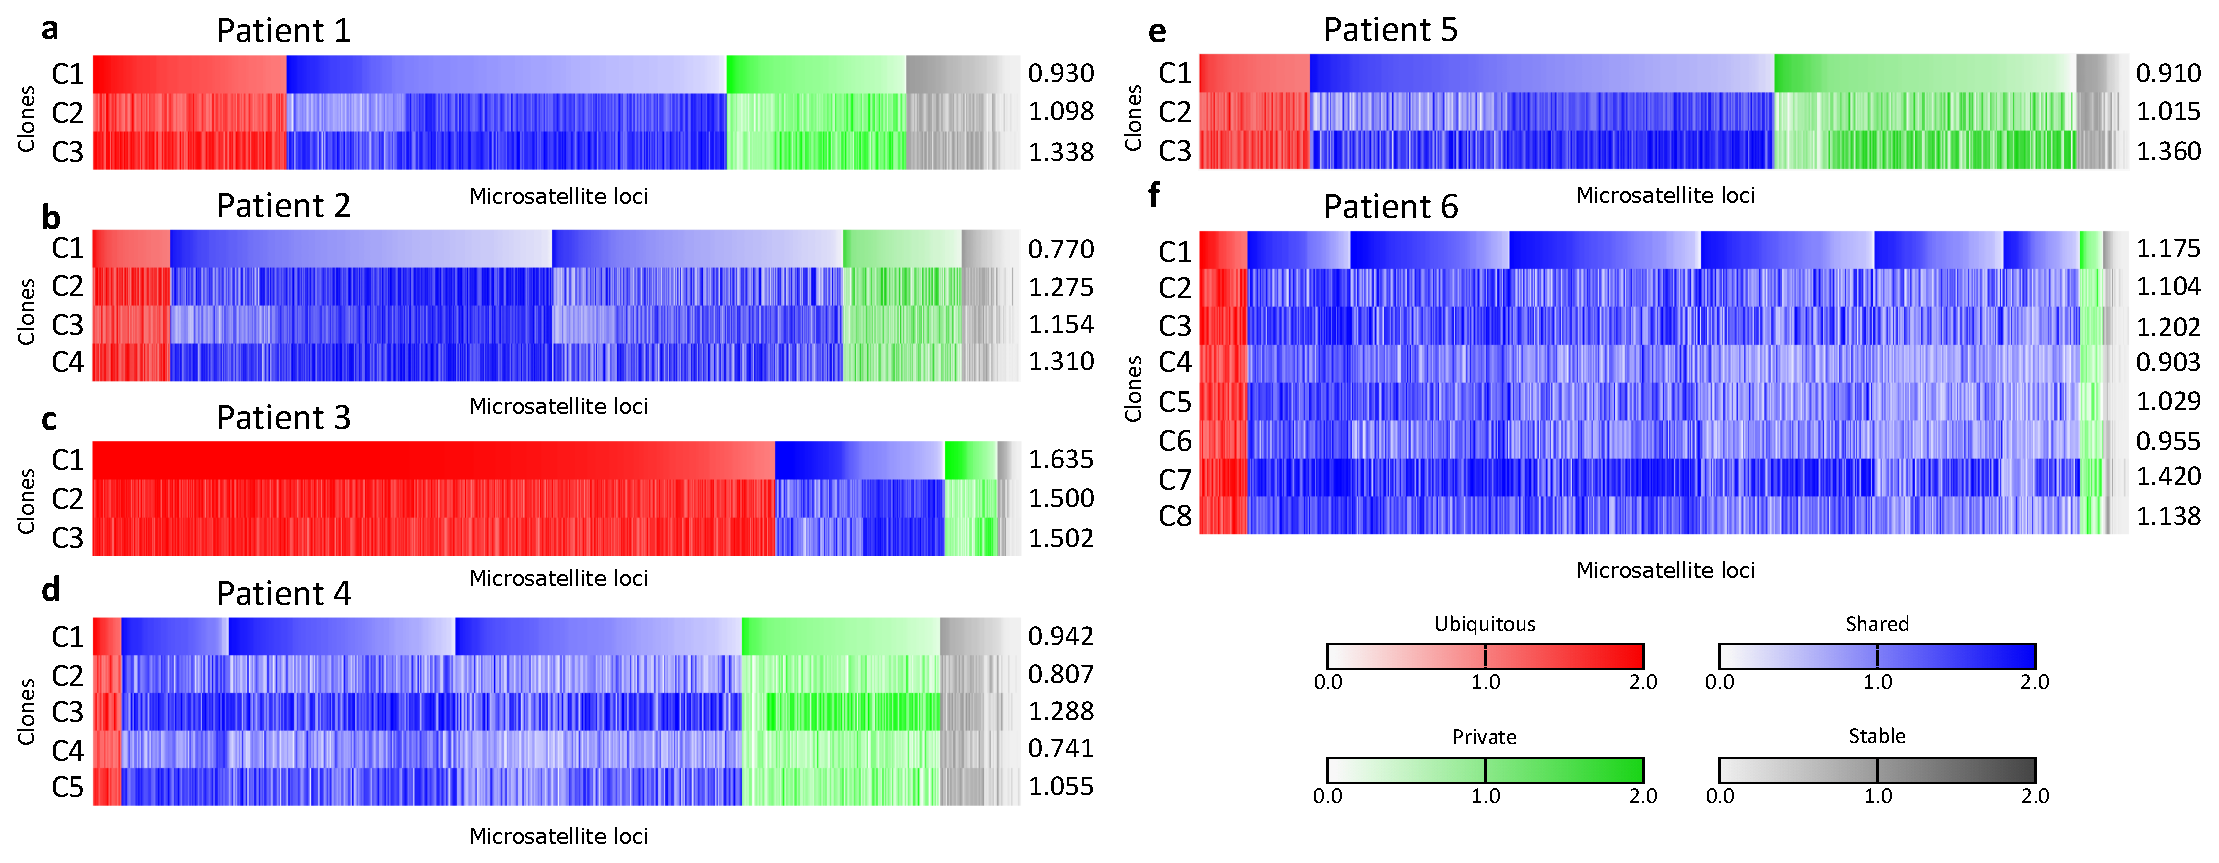
\includegraphics[width=0.98\linewidth]{images/msiclones/subclonal_ms_heatmap}
	\end{center}
	\vspace{-0.4cm}
	\caption[Subclonal MANTIS-equivalent scores.]{MANTIS scores of 714 microsatellite loci from 3 subclones in patient 1 \textbf{(a)}, 1,098 loci from 4 subclones in patient 2 \textbf{(b)}, 1,203 loci from 3 subclones in patient 3 \textbf{(c)}, 655 loci from 5 subclones in patient 4 \textbf{(d)}, 663 loci from 3 subclones in patient 5 \textbf{(e)}, and 756 loci from 8 subclones in patient 6 \textbf{(f)}. Loci with MANTIS score $\ge 1.0$ were classified as unstable. Numbers to the right of each plot indicate the MANTIS-equivalent scores of each subclone, computed by averaging across all loci.}
	\label{fig:msiclones:clonal_ms_loci}
\end{figure}

In order to interrogate microsatellites within each subclone identified by Canopy, we applied machine learning to estimate microsatellite length distributions within individual subclones (Supplemental File~S\thechapter{}.7). The hysterectomy sample from patient 5 was excluded from this analysis due to its low tumor purity (10--20\%). We computed MANTIS-equivalent measures of per-subclonal aggregate instability (Figure~\ref{fig:msiclones:clonal_ms_loci}), and found that all subclones in all patients except for P2C1 exhibited substantially increased instability compared to those patients' tumor samples. Patients 1, 2, and 6 contained direct ancestor to descendant subclonal relationships, providing a microcosm of linear evolution within otherwise branched trees. MANTIS score correspondingly increased along the P1C2--C3 and P6C6--C8--C7 lineages. Patient 2 did not follow this pattern, as P2C4 had a higher MANTIS score compared to its direct descendant P2C3. This may be explained by the fact that subclone 3 was identified in the 2015 brain sample as well as 2014 samples (Figure~\ref{fig:msiclones:clonal_fracs}), and subclone 4 was only found in a mid-2014 sample, therefore subclone 3 reflects an increased length of time for microsatellites to diverge. This may also be due to the relatively low average coverage of microsatellites by subclone 4 (29.3\texttimes{}) compared to subclone 3 (82.5\texttimes{}). Increased time for microsatellite divergence could also contribute to the increase in instability from P6C6 to P6C8.

\begin{figure}[ht]
    \begin{minipage}[b]{0.49\textwidth}
	    \begin{subfigure}{\textwidth}
	    \vspace{0.5cm}
    	    {\footnotesize
    		\begin{tabular}{r|l|l|l|l}
    			\textbf{Patient} & \textbf{Ubiq} & \textbf{Shared} & \textbf{Private} & \textbf{Stable} \\
    			\hline
    			1 & 149\ssigg & 339 & 138\ssiggg & 88\ssiggg \\
    			  & \multicolumn{1}{r|}{(130)} & \multicolumn{1}{r|}{(328)} & \multicolumn{1}{r|}{(217)} & \multicolumn{1}{r}{(39)} \\
    			\hline
    			2 & 92 & 797 & 140\ssig & 69\ssiggg \\
    			  & \multicolumn{1}{r|}{(96)} & \multicolumn{1}{r|}{(805)} & \multicolumn{1}{r|}{(173)} & \multicolumn{1}{r}{(25)} \\
    			\hline
    			3 & 884\ssiggg & 220\ssiggg & 68\ssiggg & 31\ssiggg \\
    			  & \multicolumn{1}{r|}{(808)} & \multicolumn{1}{r|}{(344)} & \multicolumn{1}{r|}{(49)} & \multicolumn{1}{r}{(2)} \\
    			\hline
    			4 & 20\ssiggg & 438\ssiggg & 140 & 57\ssiggg \\
    			  & \multicolumn{1}{r|}{(7)} & \multicolumn{1}{r|}{(479)} & \multicolumn{1}{r|}{(141)} & \multicolumn{1}{r}{(29)} \\
    			\hline
    			5 & 78 & 328\ssig & 213 & 44 \\
    			  & \multicolumn{1}{r|}{(101)} & \multicolumn{1}{r|}{(286)} & \multicolumn{1}{r|}{(230)} & \multicolumn{1}{r}{(47)} \\
    			\hline
    			6 & 39\ssiggg & 677\ssiggg & 19\ssig & 21\ssiggg \\
    			  & \multicolumn{1}{r|}{(8)} & \multicolumn{1}{r|}{(740)} & \multicolumn{1}{r|}{(7)} & \multicolumn{1}{r}{(1)}
    		\end{tabular}
		    }
		    \vspace{0.35cm}
		    \caption{}\label{fig:msiclones:shared_unstable_loci}
	    \end{subfigure}
	\end{minipage}%
	\hfill%
	\begin{minipage}[b]{0.5\textwidth}
	    \begin{subfigure}{\textwidth}
	        \centering
			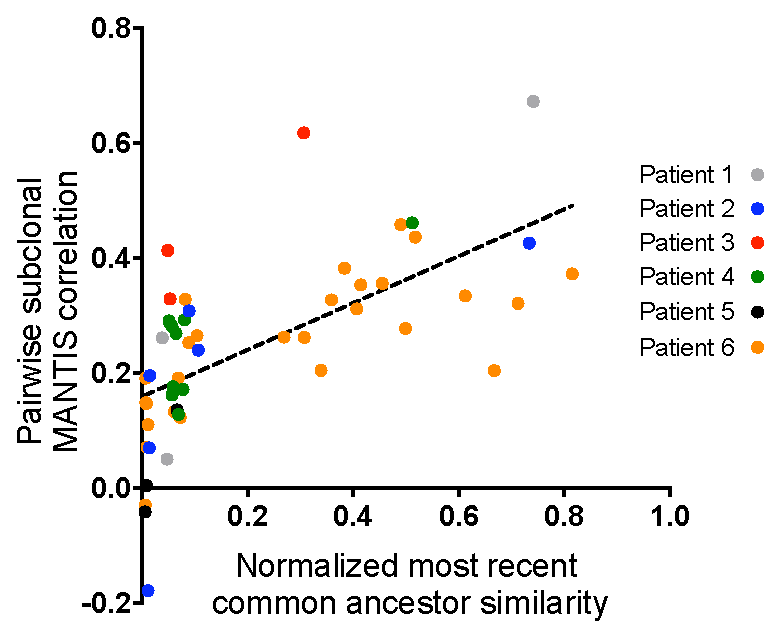
\includegraphics[width=0.98\linewidth]{images/msiclones/mrca_mantis_corr}
			\caption{}\label{fig:msiclones:mrca_corr_plot}
		\end{subfigure}
	\end{minipage}
	\vspace{-0.25cm}
	\caption[Unstable microsatellites reflect subclonal ancestry.]{(\subref{fig:msiclones:shared_unstable_loci}): Unstable microsatellites are more commonly shared among clones than expected. Ubiquitous loci are defined as unstable in all clones, shared loci unstable in more than one but not all clones, private loci unstable in one subclone, and stable loci as not unstable in any subclone. Numbers in parentheses represent the expected amount of loci in each category from each patient. Ubiq: ubiquitous. *:~$P < 0.05$. **:~$P < 0.01$. ***:~$P < 0.001$. (\subref{fig:msiclones:mrca_corr_plot}): Subclonal MANTIS score correlates with common clonal ancestry. Normalized most recent common ancestor similarity refers to the proportion of mutations in common between two clones versus the most mutated subclone (Equation~\ref{eqn:msiclones:nmrca}).}
	\label{fig:msiclones:mrca_corr}
\end{figure}

We next investigated subclonal microsatellite changes in individual loci, and found a pattern of unstable microsatellites corresponding to subclonal phylogeny. Per-locus subclonal MANTIS scores were stratified into unstable and stable groups (Section~\ref{ssec:msiclones:mantis_equiv_scores}). Loci were classified across subclones as ``ubiquitous'' if unstable in all subclones, ``shared'' if unstable in more than one but not all clones, ``private'' if unstable in only one subclone, or ``stable'' if not unstable in any subclone (Figure~\ref{fig:msiclones:clonal_ms_loci}). 397 loci were unstable in P1C2--C3 ($E \approx 336.6, P < 0.001$), consistent with their common ancestor, along with 420 loci unstable in subclones P2C2--C4 (irrespective of P2C1) ($E \approx 348.5, P \approx 0.002$). This trend was not seen for P5C2--C3, which had 267 unstable loci in common ($E \approx 264.6$, n.s.),\ possibly due to their lesser degree of common ancestry vs.\ P2C3--C4 and P3C2--C3. The overall distributions of ubiquitous\slash{}shared\slash{}private\slash{}stable loci were statistically different than expected for patients 1--4 and 6 ($P < 0.001$ for each), but not for patient 5 ($P \approx 0.09$) (Figure~\ref{fig:msiclones:shared_unstable_loci}). Patients 1--4 and 6 also possessed significantly more stable loci than expected, consistent with inheritance of unstable microsatellites rather than uniform selection of unstable loci among subclones.

\begin{figure}[htp]
	\centering
	\begin{subfigure}{0.49\textwidth}
		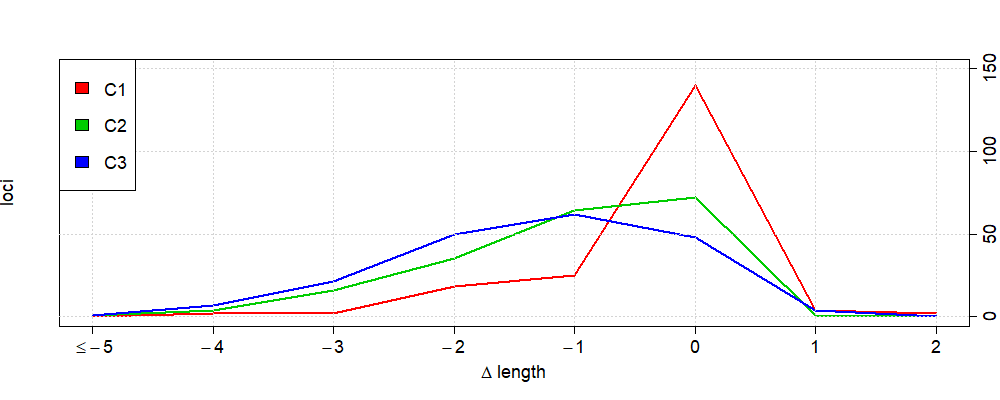
\includegraphics[width=\linewidth,keepaspectratio]{images/msiclones/patient1_median_shift}
		\caption{}\label{fig:msiclones:median_shift_1}
	\end{subfigure}%
	\hfill%
	\begin{subfigure}{0.49\textwidth}
		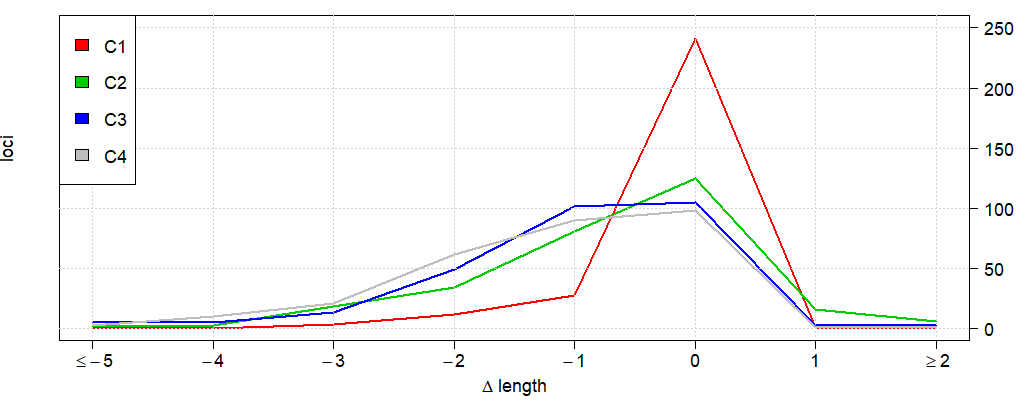
\includegraphics[width=\linewidth,keepaspectratio]{images/msiclones/patient2_median_shift}
		\caption{}\label{fig:msiclones:median_shift_2}
	\end{subfigure}
	\par
	\begin{subfigure}{0.49\textwidth}
		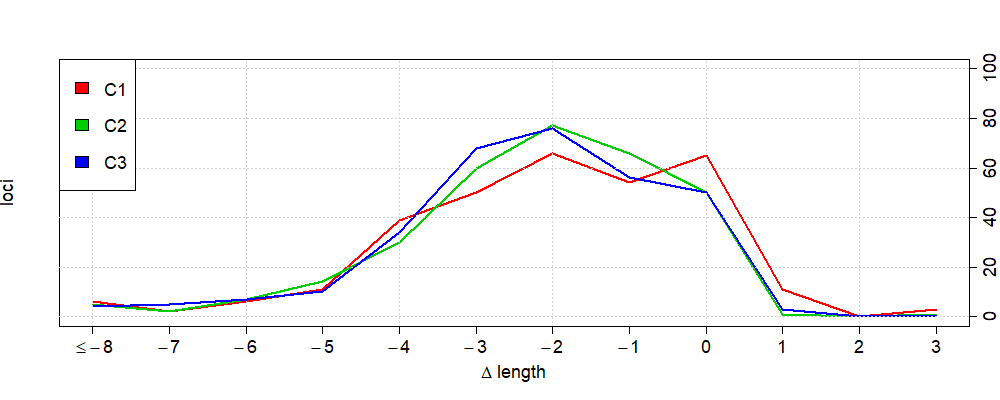
\includegraphics[width=\linewidth,keepaspectratio]{images/msiclones/patient3_median_shift}
		\caption{}\label{fig:msiclones:median_shift_3}
	\end{subfigure}%
	\hfill%
	\begin{subfigure}{0.49\textwidth}
		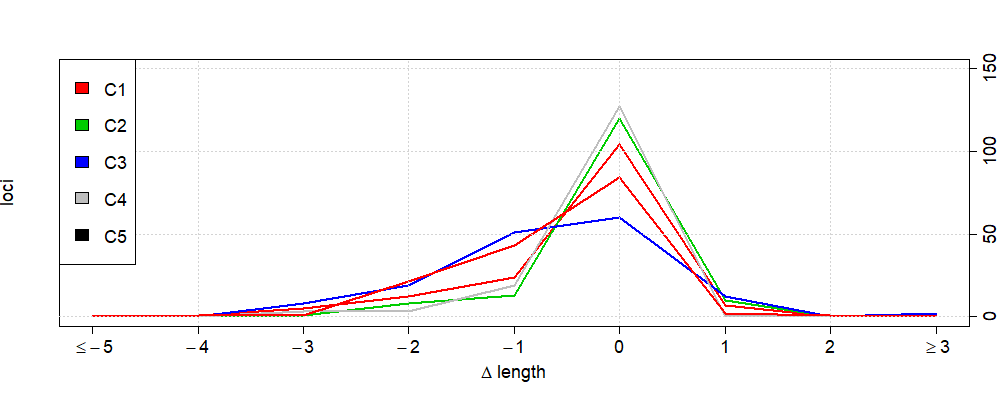
\includegraphics[width=\linewidth,keepaspectratio]{images/msiclones/patient4_median_shift}
		\caption{}\label{fig:msiclones:median_shift_4}
	\end{subfigure}
	\par
	\begin{subfigure}{0.49\textwidth}
		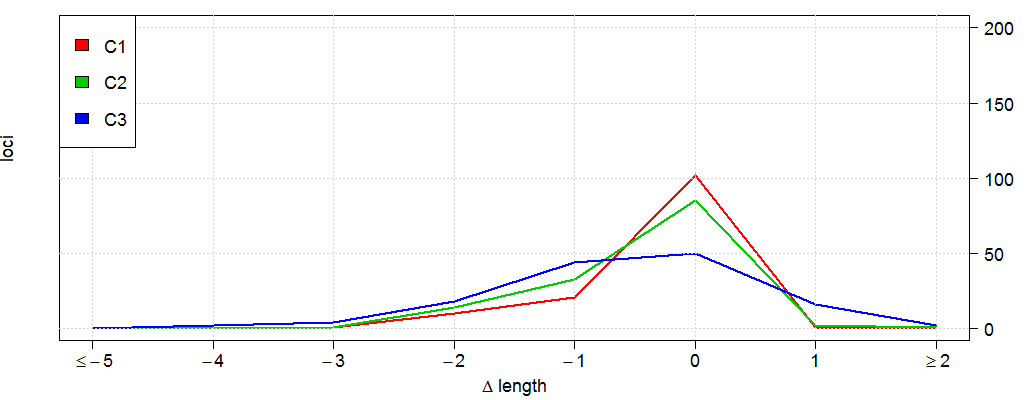
\includegraphics[width=\linewidth,keepaspectratio]{images/msiclones/patient5_median_shift}
		\caption{}\label{fig:msiclones:median_shift_5}
	\end{subfigure}%
	\hfill%
	\begin{subfigure}{0.49\textwidth}
		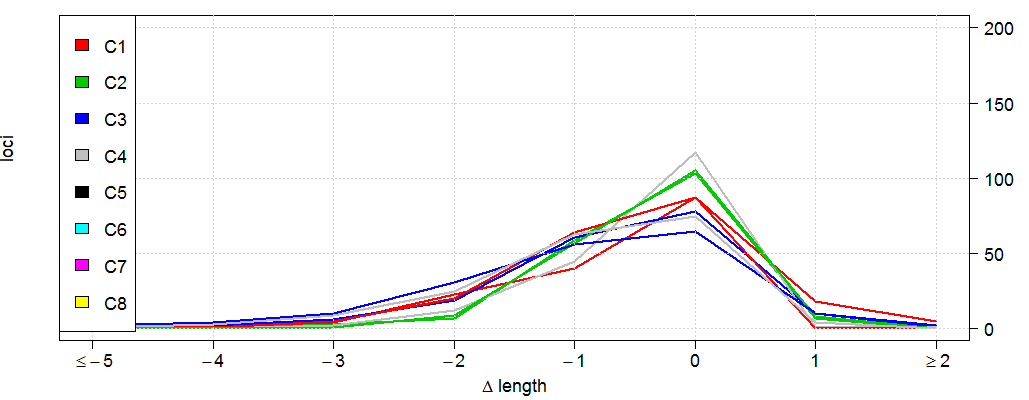
\includegraphics[width=\linewidth,keepaspectratio]{images/msiclones/patient6_median_shift}
		\caption{}\label{fig:msiclones:median_shift_6}
	\end{subfigure}
	\caption[Differences in median microsatellite loci length per subclone.]{Differences in median microsatellite loci length per subclone for single-germline locus lengths in (\subref{fig:msiclones:median_shift_1}) patient 1 (n=193), (\subref{fig:msiclones:median_shift_2}) patient 2 (n=286), (\subref{fig:msiclones:median_shift_3}) patient 3 (n=313), (\subref{fig:msiclones:median_shift_4}) patient 4 (n=153), (\subref{fig:msiclones:median_shift_5}) patient 5 (n=136), and (\subref{fig:msiclones:median_shift_6}) patient 6 (n=180). Single-germline loci were defined as loci with at least 70\% of reads supporting a single microsatellite length in the germline. Subclones are delineated by ``C\#'' in each patient.}
	\label{fig:msiclones:median_shift}
\end{figure}

Assessing loci across patients, we found that no loci were ubiquitously unstable in all six patients. Two loci were ubiquitously unstable in five patients; chr8:100287518--100287535, upstream of exon 19 of \textit{VPS13B}, a gene previously implicated in small cell lung cancer \cite{iwakawa2015}, along with chr11:102080326--102080340, downstream of exon 6 of \textit{YAP1}. We next sought to further investigate the relationship of subclonal microsatellite instability with tumor phylogeny, and found that development of instability in microsatellites follows subclonal evolution. Pooling subclones from all six patients, pairwise normalized common ancestor similarity (Equation~\ref{eqn:msiclones:nmrca}) moderately correlated with pairwise subclonal microsatellite MANTIS scores ($r = 0.638$, $P < 10^{-5}$ of regression) (Figure~\ref{fig:msiclones:mrca_corr_plot}). This was highly statistically significant ($P < 10^{-3}$, one-sided test) versus a null hypothesis of no clonal relation. This correlation rose when limited to the three patients (2, 5, 6) with samples available from multiple time points ($r = 0.712$, $P < 10^{-5}$ of regression). As our approach for subclonal microsatellite inference does not utilize phylogenetic information, this indicates its ability to recapitulate features of subclonal evolution via analysis of microsatellites independent of the SNV and CNV-based evolutionary trees from Canopy. In addition, we note that all subclones from all patients demonstrated a negative shift of median microsatellite length (average median change \mbox{-0.89}, s.d.\ 0.59), indicating that microsatellite loci tend to shorten in MMRd cells (Figure~\ref{fig:msiclones:median_shift}). This shift was less pronounced in P1C1, P2C1, P4C4 and P5C1, reflecting their lower level of microsatellite instability than other subclones. Similarly, this shift was particularly evident in patient 3's highly unstable subclones.

\section{Discussion}
\begin{figure}[ht]
	\begin{center}
		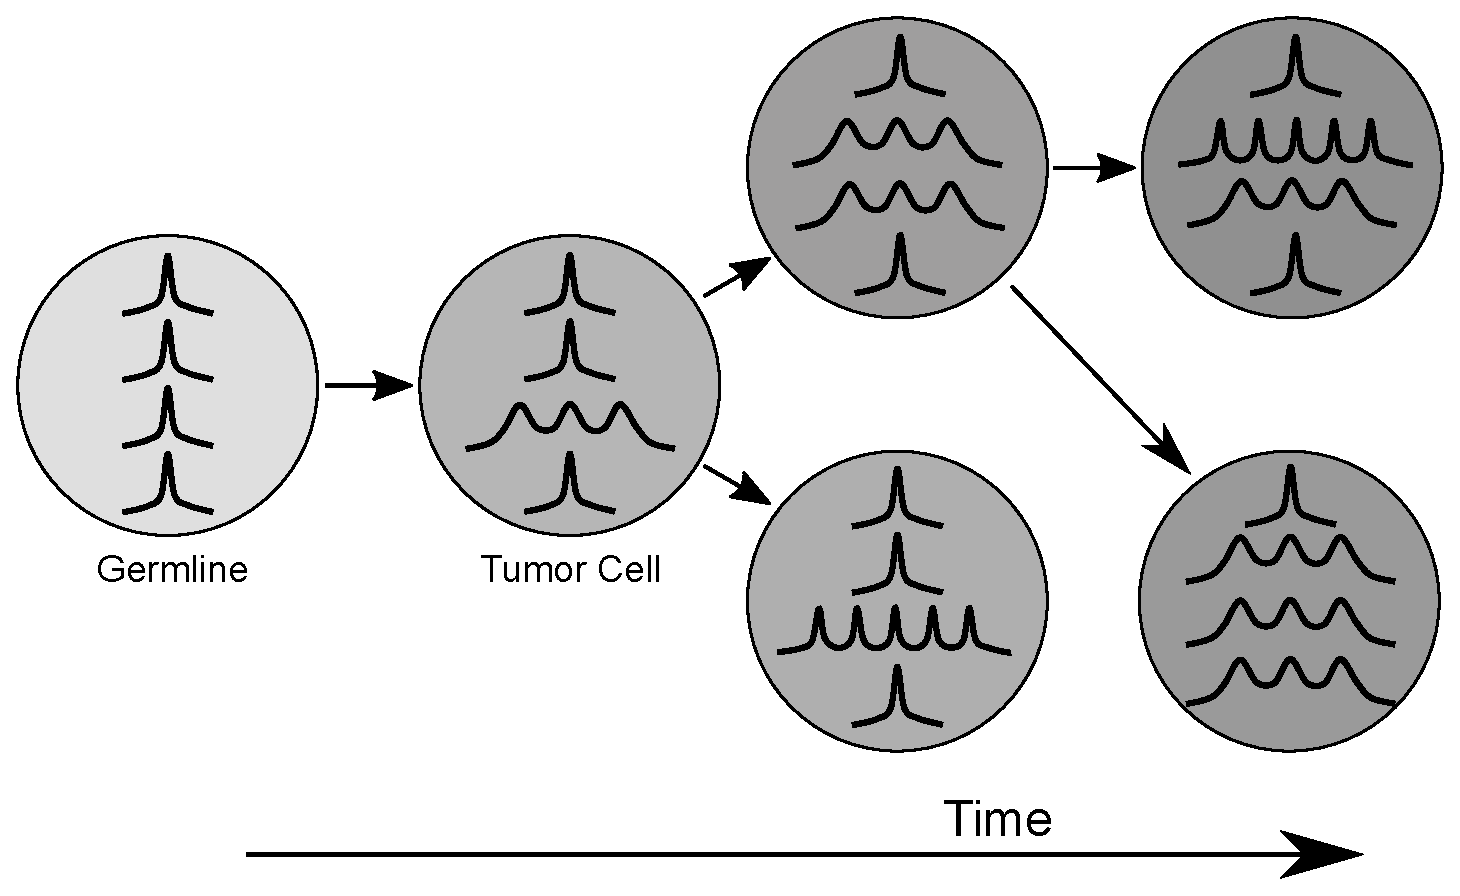
\includegraphics[width=0.7\linewidth]{images/msiclones/subclonal_ms_model}
	\end{center}
	\vspace{-0.4cm}
    \caption[Hypothesized model of clonal microsatellite instability.]{Hypothesized model of clonal microsatellite instability. In this model, mismatch repair deficiency leading to MSI develops early in tumor evolution, and is present in the founding tumor cell and all descendent subclones. As MMRd is stochastic, it introduces insertions and deletions at different loci in different cells, which fosters tumor heterogeneity. MMRd continues to cause MSI throughout the development of the cancer, which increases the level of microsatellite divergence within subclones over time. Instability at specific loci is preserved and expanded within the progeny of affected cells.}
    \label{fig:msiclones:clonal_ms_model}
\end{figure}

Tumor heterogeneity can impact diagnostic testing, therapy selection and efficacy, and tumor antigen selection \cite{mcgranahan2017}. For instance, heterogeneity has been shown to affect metastasis of colorectal cancer \cite{joung2017} and clinical outcomes in renal cell carcinoma \cite{huang2019}. Previous studies have demonstrated histologic heterogeneity within different regions of MSI-H tumors \cite{desmedt2015} and that heterogeneity impacts the accuracy of MSI-PCR and IHC \cite{chapusot2002,choi2014}. In this study, we utilized multi-sample sequencing to characterize temporal and spatial evolution of microsatellites and subclonal heterogeneity within six patients with MSI-H malignancies, modeling both acquisition of discrete mutations (SNVs\slash{}indels\slash{}CNVs) and changes in microsatellite loci. We demonstrate that microsatellite instability follows subclonal evolution, while instability at specific loci appears to be a fundamentally stochastic process (Figure~\ref{fig:msiclones:clonal_ms_model}).

Through the evaluation of 31 tumor samples in six patients, three of these patients having samples from multiple time points, we observed branching evolution, dynamic accumulation of mutations, and unique subclones. We noted a substantial level of heterogeneity in patients 1--4 and 6 (Figure~\ref{fig:msiclones:clonal_fracs}), with analysis in patient 5 likely limited by poor sample quality. Patients 2--3 and 4--6 demonstrated a branched pattern of evolution \cite{davis2017} (patient 1 having insufficient branches to classify), consistent with continued accumulation of mutations throughout the disease course and selection for subclonal driver mutations. All six patients responded to immunotherapy, and five of them displayed branching rather than neutral evolution. We speculate that the emergence of subclones containing particularly potent neoantigens was selected against by the host immune system, thus necessitating PD-1 axis inhibition to enable immunity against the subclones we detected. Branching evolution can also be driven by subclonal acquisition of mutations conferring selective advantages (such as immune evasion), enabling them to outcompete other subclones. Though five of the six patients received FOLFOX chemotherapy at some point, MMRd signatures were prominent throughout all phylogenetic trees. Taken together, these evolutionary patterns show intrinsic MMRd as a persistent generator of mutations leading to heterogeneity in MSI-H cancers.  Contrary to Sveen \textit{et al} \cite{sveen2017}, which found high proportions of truncal mutations in MSI-H tumors (median of 85\%), we made a striking observation that less than 4\% of mutations were truncal in any of these six patients. This is likely due to usage of multiple tumor samples in this study, as subclones present at similar frequencies in a single sample are difficult to separate without diversity conferred by other samples \cite{abecassis2019}. We identified multiple examples of subclones unique to particular time points and organ sites in our study, representing diversity which cannot be captured by a single sample.

We observed intra-patient tumor heterogeneity in patients with MSI-H cancers. For instance, we identified a non-hypermutated subclone P2C1 in patient 2 (TMB 2.1 mutations/Mb), which possessed a mutation in \textit{CTNNB1} but not the \textit{KRAS} mutation found in P2C2--C4. We suspect that P2C1 may represent remnants of a pre-malignant population of cells derived from the polyp, with lower levels of MSI, which eventually gave rise to cancer in this patient. P2C1 was essentially unique to the colon samples (which included the right colon primary site), and this fits with well-described genetic events for the transformation of colorectal adenoma to become carcinoma \cite{armaghany2012}, in which Wnt pathway (\textit{CTNNB1}) alterations precede \textit{KRAS} mutations. This would also be consistent with recent observations of increased MSI in endometrial carcinoma versus paired pre-malignant tissue \cite{chapel2019}. In patient 6, we detected six \textit{AR} mutations in four different phylogenetic branches, potentially accounting for resistance to multiple antiandrogen therapies during his long disease course. Multiple co-existing \textit{AR} mutations have been previously documented in MSS prostate cancer in both individual tissue samples \cite{robinson2015} and cell-free DNA (cfDNA) \cite{lallous2016,sumiyoshi2019,torquato2019}. Patients 2, 3, 4 and 6 contain genetic features typical of MSS malignancies of each type, indicating that MMRd can coexist with or potentially even account for other oncogenic pathways.

We found MSI in all subclones in all six patients, with differing levels of MSI corresponding to subclonal timing and phylogeny. Admixture of different subclones with different levels of instability has the potential to complicate NGS-based diagnostic tests for MSI, as higher tumor purity would be necessary to detect MSI in less unstable subclones. This is consistent with tumor and cfDNA testing for MSI, in which limit of detection and sensitivity decrease in samples with lower tumor content. We found that the time points of samples containing subclones substantially influenced the level of microsatellite instability. For instance, P2C1 was exclusive to earlier time points than P2C2--C4, which provides an alternative explanation for the lower level of instability in P2C1. Subclone P6C7 exhibited substantially higher microsatellite instability than P6C1--C6, likely because it was unique to the 2015 bladder biopsies and a descendant of P6C8, while other clones were observed at earlier time points. Consistent with multiple previous studies \cite{kim2013,currey2018}, we noted that unstable microsatellites preferentially shorten in length rather than expand. Notably, we found that locus-specific instability corresponded to subclonal evolution and that microsatellite analysis recapitulated phylogenetic relationships. With further refinement, this finding may enable usage of microsatellites to ``fingerprint'' tumor subclones in patients during treatment.

This study is subject to multiple limitations, primarily stemming from next-generation sequencing and clonality. Our analysis of MSI most depends on accurate estimation of subclonal prevalence. Accurate subclone detection requires precise VAFs, which in turn depend on sufficient coverage and error rates. Although we enforce a minimum coverage of 100\texttimes{} in all samples for tree-building mutations, the remaining mutations retroactively assigned to the tree can suffer from the granularity of discrete reads at low coverage. Sequencing error can also confound our deconvolution of subclonal microsatellite distributions despite the error filters provided by MANTIS, as microsatellite regions are difficult to sequence with current technology \cite{zavodna2014}. Our analysis was limited by the low quantity of tumor samples available, especially in patient 1, and in patient 5 by poor tumor cell content. Improved coverage and increased quality and quantity of tumor specimens can mitigate these issues.

The results from this study lend themselves to several avenues of further investigation. Single-cell sequencing \cite{navin2011} offers an orthogonal means of inferring phylogenetic information with fewer assumptions than bulk NGS\@. However, MSI is a property of cell populations, therefore many single cells would need to be sequenced. A hybrid approach \cite{liu2017,walter2018} employing single-cell sequencing for phylogeny and bulk NGS for microsatellites may permit increased accuracy at reduced additional expense. Inclusion of more samples from more patients would permit further investigation of the trends identified in this study, both by increasing the power to resolve subclones and by providing more exemplars of subclonal microsatellites. Furthermore, a larger sample size may permit cohort studies to identify differences in microsatellite evolution due to Lynch status, cancer type, specific MMR alterations, or other covariates. Research autopsy, as performed by our group \cite{chen2019} and others, may provide an excellent resource for high-quality tumor samples. Of clinical importance, inclusion of patients who do not respond to immunotherapies or who relapse may yield additional insights into their subclonal effects on microsatellites, especially in conjunction with emerging methods of neoantigen prediction \cite{roudko2020} and findings of microsatellite alleles relevant to host CD8\textsuperscript{+} T cell response \cite{maby2016}. An expanded mathematical model including time points could enable joint tracking of temporal and spatial evolution of microsatellite alleles, with the potential to guide therapy selection in early and late disease. Such an integrated model, building on the model developed in this study, may provide direct clinical benefit through forecasting of checkpoint inhibitor sensitivity.

In conclusion, we utilized multi-sample sequencing from multiple time points to infer subclonal phylogeny within six patients with MSI-H malignancies, identifying genetically distinct tumor subclones and branching patterns of subclonal evolution which reflect ongoing selective pressure. Improved understanding of tumor heterogeneity in MSI-H cancers has implications for improved diagnostic testing, overcoming resistance to immunotherapy, anti-tumor vaccine development, and treatment decisions over time.

\section{List of Supplemental Files}
All supplemental files are available at \url{https://github.com/rbonneville/PhD-Dissertation/}.
\begin{enumerate}
    \renewcommand*{\labelenumi}{S\thechapter{}.\arabic{enumi}. }
    \item MANTIS output for all samples from patient 1--6. Stepwise difference (column D) was used throughout this study as recommended by the authors of MANTIS\@. Row labeled ``Average'' yields per-sample MANTIS score. Also included is the list of microsatellite loci analyzed in all six patients. All genome coordinates are with reference to the hg19 reference genome. For each locus, the repeat unit is listed along with the number of occurrences in hg19, for instance \texttt{(CA)16} refers to 16 CA repeats comprising a 32 bp sequence.
    \item Summary of next generation sequencing of samples from patient 1--6, along with one normal (BN) and five tumor samples from separate patients (B1--B5) used for benchmarking our subclonal microsatellite inference algorithm. Tumor purity was estimated by a board-certified pathologist. \%100x indicates the percent of bases in the whole exome capture region covered to at least 100\texttimes{}. TMB: tumor mutational burden (mutations per megabase).
	\item Performance of subclonal microsatellite inference for 97 microsatellite loci in five tumor samples (B1--B5). Benchmarking was run five times with different random $\mathbf{P}$ matrices. Pearson correlations and associated $P$ values are listed for each locus in each run, corresponding to the accuracy with which our algorithm recovered the pure sample's microsatellite distribution for each locus and tumor sample.
    \item Annotated somatic mutations and mutational signatures identified in patients 1--6, and raw and curated CNVs identified in patient 6. SNVs and indels were called with VarScan2. Annotation was performed with ANNOVAR\@. CNVs were called using FALCON\@. Within curated calls, ``major CN'' corresponds to $\mathbf{W}_M$ in Canopy, ``minor CN'' to $\mathbf{W}_m$, ``major SD'' to $\mathbf{\varepsilon}_M$, and ``minor SD'' to $\mathbf{\varepsilon}_m$. Mutational signatures (first tab) within the COSMIC version 2 set of 30 mutational signatures were called with deconstructSigs.
    \item Fraction of each tumor subclone and normal cells within each sample from each patient as estimated by Canopy and SuperFreq. Normal represents the estimated proportion of non-tumor cells with germline DNA in each sample. Note that for patient 1, the colon polyp sample was not included in tree construction, due to its high likelihood of being drawn from a separate primary tumor than the other patient 1 samples.
    \item Mutations and mutational signatures in patient 1--6 per phylogenetic tree branch defined by Canopy or SuperFreq. Unless specified otherwise in the tab, data are from Canopy phylogenies. The six CNVs identified in patient 6 are included, along with estimated tree position and subclonal major and minor copy numbers. ``Position'' indicates the location of a mutation (SNV or indel) on the phylogenetic tree. ``Ability'' refers to the estimated ordering of mutations within a branch; mutations with higher ability occurred before those with lower ability on the same branch. Also included are mutational signatures on a per-branch basis and a per-clone basis. Branches with fewer than 50 SNVs are italicized, as the authors of deconstructSigs recommend at least 50 SNVs for signature calling. Annotation was performed using ANNOVAR\@. Ability scores were calculated using BradleyTerryScalable. Mutations were called using deconstructSigs. For patient 1, columns E--G contain alternate-supporting read counts for each mutation, H--J contain coverage depth, and K--M contain variant allele fractions. For patients 2 and 3, columns E--H contain alternate-supporting read counts for each mutation, I--L contain coverage depth, and M--P contain variant allele fractions. For patient 4, columns E--J contain alternate-supporting read counts for each mutation, K--P contain coverage depth, and Q--V contain variant allele fractions. For patient 5, columns E--I contain alternate-supporting read counts for each mutation, J--N contain coverage depth, and O--S contain variant allele fractions. For patient 6, columns E--L contain alternate-supporting read counts for each mutation, M--T contain coverage depth, and U--AB contain variant allele fractions.
	
	Tabs listed as SuperFreq (last six tabs) contain mutations (SNVs, indels, and CNVs) called by SuperFreq in patients 1--6, listed per SuperFreq subclone. Note that SuperFreq assigns mutations to vertices of the phylogenetic tree instead of edges, therefore mutations in each subclone should be interpreted as having developed in the edge leading to that subclone, and present in all descendent subclones as well.
    \item Estimated subclonal microsatellite length distributions and MANTIS scores within patients 1--6. Subclones and phylogenies identified by Canopy were used in this analysis. Each row represents the proportion of a given microsatellite length (column B) at a given locus (column A) in germline (column C) or a subclone. ``N'' corresponds to the (known) proportions of subclonal lengths from sequencing of the matched normal. To compute MANTIS scores, a stepwise distance metric was used, consistent with the metric used for per-sample microsatellite analysis in this study. The row labeled ``Average'' yields per-subclone MANTIS score.
\end{enumerate}

\section*{Acknowledgements}
We are grateful for administrative support from Jenny Badillo, the Comprehensive Cancer Center at The Ohio State University, computational resources from the Ohio Supercomputer Center (OSC), community support from Pelotonia, technical assistance with SuperFreq from Gregory Wheeler, PhD (Nationwide Children's Hospital, Columbus, OH), and most importantly the patients included in this study and their families.

Sequencing reads from all six patients in this cohort have been deposited in dbGaP (\url{https://ncbi.nlm.nih.gov/gap}) under accession number phs001925.v1.p1.
